% !TEX encoding = UTF-8 Unicode
\newcommand{\red}[1]{\textcolor{red}{#1}}
\newcommand{\blue}[1]{\textcolor{blue}{#1}}
\newcommand{\green}[1]{\textcolor{green}{#1}}
\newcommand{\purple}[1]{\textcolor{purple}{#1}}

\linespread{1.7}
\chapter{0-5 Hz Deterministic 3D Ground Motion Simulations for the 2014 La Habra, California, Earthquake}
\linespread{2.0}
%\newrefsection
\label{chap:highf}

\graphicspath{{/Users/zhh076/work/PhD_way/high_f/}}

We have simulated 0-5 Hz deterministic simulations for the 2014 $M_w$ 5.1 La Habra, CA, earthquake in a mesh from the Southern California Earthquake Center Community Velocity Model Version S4.26-M01 and a finite-fault source. Our simulations include statistical distributions of small-scale crustal heterogeneities (SSHs), frequency-dependent attenuation $Q(f)$, effects of near-surface low velocity material, and surface topography. Strong motion data at 259 sites within an 148 km by 140 km area are used to validate our simulations.  Amplification from the near-surface low-velocity soil column appears from about 0.3 Hz, increasing to factors of 2-3 approaching 5 Hz. We find that a high-frequency power law for $Q(f)=Q_o f^{\gamma}$ with $\gamma$ of 0.4-0.6 provides optimal fit to the data. Topography, and to a lesser extent SSHs, predominantly decreases the peak velocities and significantly increase the duration. A weathering layer with realistic near-surface low velocities is found to enhance the amplification at mountain peaks and ridges. Our results show that the effects of near-surface low-velocity material, topography, SSHs and $Q(f)$ become increasingly important and should be included as frequencies increase. The results provide guidance on the importance of the different features controlling high-frequency seismic hazard analysis.


%%%%%%%%%%%%%%%%%%%%%%%%%%
\section{Introduction} \label{highf:intro}
It is the ultimate goal for ground motion modelers to deliver their results to engineers and see their work used in applications beneficial for society, such as structural design. This is particularly useful in cases of infrequent observations, such as large magnitude events at small distances from the fault, where simulations may provide a viable alternative to data. Deterministic ground motion predictions, including features such as three-dimensional (3D) velocity structure and frequency-independent anelastic attenuation are now routinely produced for frequencies up to about 1 Hz with generally satisfactory fit to recorded data \citeg{gravesSimulatingSeismicWave1996,olsen2009shakeout,roten3DSimulationsEarthquakes2012,}. These simulations have proved to be useful in public earthquake emergency response and seismic hazard management \citep{gravesBroadbandGroundMotionSimulation2010}, and complementing empirical ground motion prediction models in regions with sparse stations coverage \citeg{dayModelBasinEffects2008}.

While the results of these low-frequency simulations are promising, structural engineers need ground motions with signal content up to 5 Hz and higher for design purposes. Hybrid techniques, combining deterministic low-frequency and stochastic high-frequency signals \citeg{olsen2015sdsu,gravesKinematicGroundMotion2016} can be used to generate synthetic seismograms with frequency content up to 10 Hz and higher. However, simulating both the lower and higher frequency content using a deterministic approach has the potential to lower part of the epistemic uncertainty in the resulting ground motion estimates. In this study we investigate the feasibility of increasing the highest frequency for the deterministic ground motion predictions to 5 Hz, using simulations and data for the 2014 $M_w$ 5.1 La Habra, CA, earthquake. The La Habra event was chosen due to an abundance of records available in the greater Los Angeles area, while ground motions can be considered linear due to its relatively small magnitude.


As frequencies increase above about 1 Hz, features with increasingly small length scales become important to realistically predict deterministic ground motions. For example, small-scale complexity of both the source and surrounding media, on the order of 10-100s of meters, is expected to increasingly affect the ground motion predictions at higher frequencies. Frequency-independent anelastic attenuation, often chosen as proportional to the local velocity structure \citeg{gravesBroadbandGroundMotionSimulation2010} is usually a good approximation for lower frequencies \citep[e.g., up to ~1 Hz][]{liu1976velocity,fehler1992separation}. However, models of frequency-independent anelastic attenuation appear to be inconsistent with seismic records at higher frequencies where regional studies indicate that larger Q values may be more accurate \citeg{withersMemoryEfficientSimulation2015}. Finally, ground motion simulations often artificially truncate the lowest near-surface velocities due to computational limitations, which may be a reasonable approximation for lower frequencies \citeg{olsenEstimationLongPeriodSec2003}. However, stronger effects from this near-surface material emerge as frequencies increase and wavelengths decrease \citeg{pitarka2009simulating,imperatoriBroadbandNearfieldGround2013}. Here, we quantify the effects of all of these features in our 3D simulations of the La Habra event.

In southern California, two 3D state-of-the-art velocity models, namely the Community Velocity Models (CVM) versions S and H have been developed through the Southern California Earthquake Center (SCEC). These CVMs have been validated against ground motion data in a series of studies \citeg{tabordaEvaluationSouthernCalifornia2016,savranGroundMotionSimulation2019,laiShallowBasinStructure2020}, where conclusions often point to inaccuracies in the velocity structure, in particular for the near surface material. \citet{elyVs30derivedNearsurfaceSeismic2010} proposed a method to calibrate the near-surface material based on estimates of the time-averaged velocity in the upper 30 m ($V_{S30}$), and later improved by \citet{huCalibrationNearsurfaceSeismic2021}, specifically for sites with poor constraints in shallow velocities. In this study, we use the SCEC CVM-S4.26-M01 with the near-surface $V_S$ tapering method proposed by \citet{huCalibrationNearsurfaceSeismic2021} (hereafter referred to as CVM-S).

The effects of irregular surface topography on ground motions also play an increasingly large role as frequencies increase \citeg{liuScatteringSeismicWaves2020}. In addition, in recent studies, theoretical and numerical methods have helped clarify the interaction between seismic waves and topography \citep[mainly scattering and trapping of waves, e.g.,][]{imperatoriRoleTopographyLateral2015,takemura2015scattering,rodgersBroadband04Hz2018}, as well as describing the characteristic effects on ground motions. Some of the most notable effects of topography are listed in the following. (1) Amplification tends to occur at the top of relatively steep slopes for waves with comparable wavelength to the size of the topographic features; on the other hand, deamplification tends to occur at low-elevation areas \citep{trifunacAnalysisPacoimaDam1971,booreNoteEffectSimple1972,spudichDirectionalTopographicSite1996,bouchonSeismicResponseHill1996,assimakiSoilDependentTopographicEffects2005}. Amplification can range up to a factor of 10 or more between the crest and base of a topographic feature \citep{davisObservedEffectsTopography1973,geliEffectTopographyEarthquake1988,umedaHighAccelerationsProduced1987,gaffetSiteEffectStudy2000}. (2) The amplification at mountain tops is systematically larger for incident S compared with P waves, and such difference diminishes when the slope decreases or the incidence angle increases \citep{bardDiffractedWavesDisplacement1982}. (3) Body waves and surface waves are strongly scattered by irregular topography, thus reducing ground motion amplitudes while prolonging the shaking durations \citep{sanchez-sesmaDiffractionSVRayleigh1991,leeEffectsRealisticSurface2009}. (4) Topography tends to disrupt the coherency of high-frequency ground motion and thereby distorts the S-wave radiation pattern \citep{imperatoriRoleTopographyLateral2015}. Notably, 3D models of the topography are necessary to capture the amplification effects, as noted in two-dimensional (2D) simulation results \citep{geliEffectTopographyEarthquake1988,bouchonSeismicResponseHill1996}. While geometrical characteristics, such as smoothed curvature and relative elevation, have been explored to approximate topographic effects \citeg{maufroyFrequencyScaledCurvature2015,raiEmpiricalTerrainBasedTopographic2017}, they require critical parameter constraints based on local velocity and target frequency, and thus difficult to be generalized for broadband studies.

It should be noted that previous studies discussed above included only a subset of the model features deemed to be affecting high-frequency ground motions, or omitted validation of the results. In this study, we simulate ground motions for frequencies up to 5 Hz in the widely-tested SCEC CVM-S4.26M01 including high-resolution topography and compare to strong-motion data for the 2014 $M_w$ 5.1 La Habra, CA, earthquake, in order to constrain the relative contribution of topography, SSHs, and $Q(f)$. Our paper is organized as follows. We first describe the velocity model, simulation parameters, processing of the synthetic and recorded ground motions, and source description. Then the relative effects of model features such as topography, shallow near-surface velocities, small-scale heterogeneities, and $Q(f)$ will be quantified through goodness-of-fit (GOF) measures between synthetics and data, as guidelines for future simulations. Finally, we discuss future research directions based on our results.



%%%%%%%%%%%%%%%%%%%%%%%%%%%%%%%
\section{Computational Aspects}\label{approach}

In this section we describe the simulation method and model setup, and summarize the features included in our model. In addition, we outline the processing parameters for simulations and data, and introduce our goodness-of-fit (GOF) measures to validate our results.

\subsection{Numerical method for simulating ground motions}
We use the staggered-grid finite-difference (FD) code AWP-ODC \citep[Anelastic Wave Propagation, Olsen-Day-Cui, from the authors of the code, hereafter denoted by AWP;][]{cuiScalableEarthquakeSimulation2010}, which is $4^{\text{th}}$-order accurate in space and $2^{\text{nd}}$-order accurate in time, to generate ground motion predictions for the La Habra event. AWP has been adapted to GPU accelerators for kinematic sources \citep{cui2013physics}, and provides support for frequency-dependent viscoelastic attenuation \citep{withersMemoryEfficientSimulation2015} and topography using a curvilinear grid \citep{oreillyHighorderFiniteDifference2021}. 

The accuracy of AWP has been thoroughly verified. For example, large-scale earthquake simulations in realistic 3D earth models with strong heterogeneities and complex finite-fault source descriptions \citep{bielakShakeOutEarthquakeScenario2010,bielak2016verification}, revealed good agreement between AWP, another staggered-grid FD code and a finite-element code. The DM method implemented in the scalable GPU version of AWP was verified against uniform mesh solutions for the $M_w$ 5.1 La Habra earthquake \citep{rotenHighfrequencyNonlinearEarthquake2018}. The implementation of frequency-dependent anelastic attenuation was tested by \citet{withersMemoryEfficientSimulation2015} against a frequency-wavenumber solution, and the accuracy of the curvilinear topography implementation \citet{oreillyHighorderFiniteDifference2021} was verified against SPECFEM3D \citep{komatitschSpectralelementSimulationsGlobal2002}.


\subsection{Computational Domain}
We used a model domain of lateral dimensions 148 km by 140 km, rotated 39.9$^{\circ}$ clockwise with a depth extent of 60 km. The mesh was extracted from the SCEC CVM-S4.26-M01, an updated version of the original CVM-S4 model \citep{magistraleSCECSouthernCalifornia2000,kohlerMantleHeterogeneitiesSCEC2003} with iterative 3D full tomography inversions in Southern California \citep{leeRapidFullwaveCentroid2011}. The SCEC Uniform Community Velocity Model software framework \citep[V19.4][]{smallSCECUnifiedCommunity2017} was used for the extraction of seismic P-wave velocity ($V_P$), $V_S$ and the material density. The choice of CVM-S4.26-M01 (hereafter abbreviated with CVM-S) for this study was based on the results by \citet{tabordaEvaluationSouthernCalifornia2016} who concluded from a comprehensive validation of four velocity models with 30 earthquakes in the greater Los Angeles region that this model consistently yielded the best fit to ground motion data using a variety of metrics.

\subsection{Small-scale Heterogeneities}
Small-scale (on the order of tens to hundreds of meters) crustal heterogeneities are known to exist in nature but are insufficiently resolved in state-of-the-art velocity models. Instead, small-scale heterogeneities are commonly included in numerical simulations via statistical models of property fluctuations \citeg{imperatoriBroadbandNearfieldGround2013,savranGroundMotionSimulation2019}. Here, we superimpose a statistical model of velocity and density perturbations onto CVM-S, defined via a Von Karman shape function \citep{frankelFiniteDifferenceSimulations1986}:

\begin{equation}\label{eq:highf-1}
  \Phi_{v, a}(r)=\sigma^{2} \dfrac{2^{1-v}}{\Gamma(v)}\left(\dfrac{r}{a}\right)^{v} K_{v}\left(\dfrac{r}{a}\right)
\end{equation}

\noindent which has Fourier transform:

\begin{equation}\label{eq:highf-2}
  P(k)=\dfrac{\sigma^{2}(2 \sqrt{\pi} a)^{E} \Gamma(v+E / 2)^{v+E / 2}}{\Gamma(v)\left(1+k^{2} a^{2}\right)}
\end{equation}
\noindent in which $k$ is the wave number and $E$ is the Euclidean dimension, $\Gamma$ denotes the Gamma function, and $K$ stands for the modified Bessel function of the second kind with order $\nu$. The parameters of the Von Karman autocorrelation function include correlation length $a$, standard deviation $\sigma$ and Hurst number $\nu$. This approach generates a random field with zero mean, and the desired standard deviation is guaranteed by scaling the random variable at each computational node. We used a fixed Hurst number of 0.05 and introduced elliptical anisotropy with a ratio of horizontal-vertical correlation lengths of 5. We tested correlation lengths between 100-500 m, and standard deviation of 5\% and 10\%, based on previous studies in Southern California \citeg{nakataStochasticCharacterizationMesoscale2015,savranModelSmallscaleCrustal2016}. In our model, the random perturbations extend to a depth of 7.5 km, and then linearly tapered to a standard deviation of 0 at 10 km depth \citep{olsen2018constraints}. \Cref{fig:highf-2} shows an example realization of small-scale heterogeneities, compared to the original CVM-S in terms of $V_S$ at the surface.

\subsection{Topography}
While the basins of the greater Los Angeles region, including near the epicentral area of the La Habra event, are characterized by relatively flat topographic relief, the San Gabriel and Santa Ana Mountains bound the area to the North and East, respectively (see \cref{fig:highf-1}). To quantify the effects of topography on ground motions from the La Habra event, we use the curvilinear grid approach by \citet{oreillyHighorderFiniteDifference2021}. In this version of AWP, surface topography is incorporated by stretching the computational grids in the vertical direction, while keeping the horizontal grid spacing unchanged, so that the surface grid locations conform to the shape of the topography. We include surface topography into our model domain via the $\dfrac{1}{3}$ arc-second resolution Digital Elevation Model in southern California from the U.S. Geological Survey (USGS).

\subsection{Frequency-Dependent Attenuation}
Anelastic attenuation is needed for accurate simulation of seismic wave propagation through earth models at distances further than the dominant wavelength to account for the loss of intrinsic energy. Frequency-independent attenuation, resulting in identical seismic energy loss per cycle across a frequency bandwidth, has successfully been used to validate ground motion recordings for frequencies up to about 1 Hz \citeg{olsenEstimationLongPeriodSec2003,graves2004observed}. However, as frequencies increase above about 1 Hz, data often supports frequency-dependent $Q$ \citeg{raoof1999attenuation,eberhart2014imaging,wangUsingDirectCoda2017}. To address these findings, \citet{withersMemoryEfficientSimulation2015} developed an efficient coarse-grained memory variable approach to model frequency-dependent attenuation using a power law formulation

\begin{equation}\label{eq:highf-3}
  Q(f)=Q_{0} *\left(\dfrac{f}{f_{0}}\right)^{\gamma}, \quad f \geq f_{0},
\end{equation}
\noindent where $Q_0$ is a frequency-independent $Q$ value applied for $f<f_{0}$.  \citet{withersMemoryEfficientSimulation2015} and \citet{savranGroundMotionSimulation2019} found that $\gamma$ values of to 0.6-0.8 produced the best fit to seismic records of the 2008 Chino Hills, CA, earthquake.

A widely-used parameterization of $Q_0$ is proportional to local seismic velocity, with separate values $Q_{0P}$ and $Q_{0S}$ for $V_P$ and $V_S$ quality factors, respectively, producing an expected stronger attenuation for lower velocity material pointed out by \citet{haukssonAttenuationModelsThree2006}. \citet{taborda2014ground} revised the formula expressed by \citet{brocher2008compressional} and applied a $6^{\text{th}}$-order polynomial function for $Q_{0S}$ from $V_S$, and $Q_{0P}=\dfrac{3}{4}\left(V_P/V_S\right)^2Q_{0S}$. We test a variety of these parameterizations of $Q_0$ for the La Habra event.

\subsection{Near-surface Geotechnical Layer}
CVM-S includes geotechnical data which integrates geology and geophysics data from surficial and deep boreholes, oil wells, gravity observations, seismic refraction surveys and empirical rules calibrated based on ages and depth estimates for geological horizons in southern California \citep{magistraleGeologybased3DVelocity1996,magistraleSCECSouthernCalifornia2000}. While recent validation studies, such as \citet{tabordaEvaluationSouthernCalifornia2016}, have shown that the basin structure included in CVM-S is reasonably accurate, unrealistically large surface rock site velocities (see \Cref{fig:highf-2}) motivated the method by \citet{elyVs30derivedNearsurfaceSeismic2010} to reduce the $V_S$ in the top 350 m based on available $V_{S30}$ values. Recently, \citet{huCalibrationNearsurfaceSeismic2021} proposed a method to further adjust the near-surface structure to a depth of 1000 m, resulting in an improved fit between simulated and recorded Fourier spectra below 1 Hz for the La Habra earthquake, which will be used in this simulations in this study.

\subsection{Ground Motion Simulations}
Table 1.1 lists the parameters used in our simulations. All simulations have the same duration of 120 s and resolve wave propagation up to $f_{max}=5$ Hz by at least 5 points per minimum S-wavelength. We use AWP-topo that supports uniform regular, curvilinear mesh to model wave propagation in composite models including topography and other features, with the minimum $V_S$ clamped at 500 m/s to alleviate computational cost. We use a kinematic source generated following \citet{gravesKinematicGroundMotion2016}, which creates finite-fault rupture scenarios with stochastic characteristics optimized for California events. The focal mechanism was taken from the U.S. Geological Survey \citep[strike=233$^\circ$, dip=77$^\circ$, rake=49$^\circ$; ][]{usgsEarthquakeEventsFocal2014} with a moment magnitude 5.1 and a fault area of 2.5 km x 2.5 km. 


\subsection{Data Processing}
259 strong-motion seismic stations were used to validate the simulations. The strong motion recordings (velocity time series) are obtained from SCEC (F. Silva, Personal Communication, 07/2020), with hypocentral distance up to 90 km and signal-to-noise ratio above 3 dB. The processing procedure included the following steps: (1) low-pass filtering of the time series below 10 Hz using a zero-phase filter; (2) interpolating the time series linearly to a uniform time step; (3) tapering of at the last 2 seconds using the positive half of a Hanning window; (4) zero padding the last 5 seconds; (5) filtering the seismograms to the desired frequency, and (6) converting velocities to accelerations by a time derivative. Except for the initial 10 Hz low-pass filter, all filters used a low-cut frequency of 0.15 Hz to avoid noise interference. $4^{\text{th}}$-order Butterworth filters were used in all cases. Finally, our horizontal synthetic seismograms were rotated 39.9$^\circ$ clockwise to minimize the computational requirements needed to include all seismic stations.

\subsection{Goodness of fit criteria}
We used a modified subset of the goodness-of-fit (GOF) metrics proposed by the methods of \citet{andersonQuantitativeMeasureGoodnessOfFit2004} and \citet{olsenGoodnessoffitCriteriaBroadband2010} developed for the comparison of broadband seismic traces (0 to 10+ Hz). The method includes 10 different metrics, from which we selected 7, namely peak ground velocity (PGV), peak ground acceleration (PGA), energy duration (DUR), cumulative energy (ENER), response spectral acceleration averaged between 0.1 and 10 s (RS), and smoothed Fourier amplitude spectrum (FAS), as well as one additional metric, Arias intensity (AI), to compute our GOF scores. We computed the SA at frequencies linearly spaced from 0.2 to 5 Hz. Cumulative energy is calculated as $E N E R=\int v(t)^{2} d t$. Both ENER and DUR are defined on the interval between the arrival of 5 and 95 percent of the total energy. Arias intensity describes the cumulative energy per unit mass \citep{arias1970measure}, and is defined as $AI=\dfrac{\pi}{2 g} \int a(t)^{2} d t$, where $a(t)$ is the acceleration time series, and $g$ is the gravitational acceleration. 

The GOF score for each metric is defined as
\begin{equation}\label{qe:highf-4}
  G_{\text {metric }}=10 \operatorname{erfc}\left(\dfrac{2|x-y|}{x+y}\right).
\end{equation}
\noindent where $x$ and $y$ are two positive scalars from the selected metrics. $G_{\text {metric}}$ is computed for each metric and combined into a weighted average using all 3 components. We used weights of 0.5, 0.5, 1, 0.5, 0.5, 1, and 1 for for PGV, PGA, DUR, AI, ENER, RS, and FAS, where reduced weights are chosen due to correlation between metrics \citep{olsenGoodnessoffitCriteriaBroadband2010}. The GOF score for the entire simulation is calculated as the average of $G_{\text {station }}$ across all 259 stations. GOF values between two signals above 4.5 and 6.5 are considered fair and very good fit, respectively.

\section{Results}
\subsection{Source Models}
Due to the stochastic characteristics of the kinematic source generator by \citet{gravesKinematicGroundMotion2016}, a series of 40 source realizations with different random seeds are evaluated based on comparisons between spectral accelerations with records at stations with epicentral distance of 31 km or less (R. Graves, Personal Communication, 03/04/2020). The 40 source models were rated based on the average absolute bias between synthetics and data up to 5 Hz for the median pseudo-spectral acceleration rotated over all azimuths (rotD50), from which we selected the three best performing source descriptions with hypocentral depths at 5, 5.5 and 6 km (see \cref{fig:highf-3}). The rupture duration of the source descriptions is less than 2 s and sampled at an interval of 0.001 s, identical to the time step used in our simulations. The three sources tend to generate overall similar patterns of PGV within the same bandwidth of low (< 2.5 Hz) or high (> 2.5 Hz) frequencies (\cref{fig:highf-4}). Based on this result, we carry out our analysis with Source 1 only in order to limit the computational requirements.

\subsection{Minimum \textbf{$V_S$}}
Southern California features several low-velocity basins where the minimum (surface) $V_S$ in CVM-S can be much lower than the minimum value of 500 m/s that we imposed in our models (see \cref{tab:highf-1}). As previous studies have pointed out, soft soils, characterized by lower $V_S$, have been found to generate significant amplification of the ground motions \citeg{anderson1984model}. Reducing the minimum $V_S$ will, however, increase the computational cost for the series of 3D numerical simulations needed in our analysis beyond the available resources. For example, clamping the minimum $V_S$ at 200 m/s instead of 500 m/s requires about 40 times more node hours for a single simulation. 

For this reason, we use a computationally much less expensive 1D method, which models vertically-incident SH waves in a horizontally-layered halfspace \citeg{dayRMSResponseOnedimensional1996,thompsonTaxonomySiteResponse2012}, to account for effects of the material with $V_S$ less than 500 m/s. At each site, we calculated the response from two 1D models, one using the velocity profile from our models, and the other using the same profile but with minimum $V_S$ clamped at 500 m/s. In this way, the ratio of the two 1D results characterizes the effects of the material with $V_S$ less than 500 m/s, which is then convolved with our 3D simulations. Because the SH1D method considers SH waves only, we will apply this calibration to horizontal components only. This procedure is encouraged by the results of 3D simulations minimum $V_S$ of 200 m/s and 500 m/s up to 2 Hz using the domain in \cref{fig:highf-1}, showing negligible differences on the vertical component (\cref{fig:highf-S1}).

\Cref{fig:highf-5} illustrates the results of applying the SD1D method low-velocity correction for an example site. The two profiles show similar SH1D responses below about 0.3 Hz, above which the SH1D response ratio slowly trends upward with frequency, depicting the amplification from the material with $V_S$ less than 500 m/s. The PGV of the horizontal synthetic with the correction is increased by 32\% \Cref{fig:highf-5}c relative to that with $V_S$ clamped at 500 m/s. The correction leaves the shape of the waveform almost unchanged. The smoothed Fourier spectra (\Cref{fig:highf-5}d) further suggests that clamping $V_S$ at 500 m/s may be reasonable for frequencies up to 0.8-1 Hz. Similar effects are observed for all profiles with near-surface velocity lower than 500 m/s, and we therefore apply this technique to all our 3D simulations with minimum $V_S$ clamped at 500 m/s.


\subsection{Reference Model Response}
\Cref{fig:highf-6} shows a comparison between PGVs extracted from records and synthetics for a simulation with source 1, CVM-S including topography, $Q(f)=0.1f^{0.6}$, $Q_P=2Q_S$, shallow velocity tapered down to 1000 m \citep{huCalibrationNearsurfaceSeismic2021}, and no small-scale heterogeneities added, which is our reference case for low frequencies (0.15-2.5 Hz) and high frequencies (2.5-5 Hz). The minimum $V_S$ is truncated at 500 m/s (at which $V_P$ is calculated from the $V_P/V_S$ ratio in CVM-S, and density is unchanged), often necessitated by limitations of computational resources. While the overall PGV distributions are similar, the reference model tends to predict larger values to the south and west of the source within 40 km distance, especially at high frequencies. On the other hand, the simulation slightly underpredicts the PGVs beyond 40 km at frequencies above 2.5 Hz. The overprediction in the nearfield and small underprediciton in the farther field at high frequencies indicates more than expected seismic energy is trapped within the Los Angeles Basin (LAB) bounded by San Bernardino and Santa Ana Mountains (see \cref{fig:highf-2}a for location). The overprediction within 40 km may suggest a lower $Q$ within the LAB, as hypothesized by \citet{houghAttenuationAnzaCalifornia1988} and examined by \citet{withersValidationDeterministicBroadband2019} that a frequency-dependent low $Q$ layer improves the prediction of site effects.


\subsection{Topography}
In this section we investigate the effects of topography, which are often ignored in numerical simulations \citeg{graves2004observed,olsenStrongShakingAngeles2006,savranGroundMotionSimulation2019}. Our analysis of topographic effects uses a reference model with topography removed.
\Cref{fig:highf-7} shows the percent difference between models with and without topography for PGV, DUR and AI for bandwidths of 0.15-1 Hz, 1-2.5 and 2.5-5 Hz. It is clear that topography complicates the wavefield pattern significantly, even at frequencies below 1 Hz in terms of DUR and thus AI. Consistent with previous studies \citeg{hartzell1994initial, leeEffectsRealisticSurface2009}, we observe a weak deamplification of PGV below 1 Hz in basin areas, while that mountain peaks and ridges may amplify PGV by less than 50\%. In addition, we find that PGV is reduced by about 30\% in the Chino Basin and northwest of San Gabriel Mountains. These results are in agreement with \citet{maEffectsLargeScaleSurface2007} who found that the San Gabriel Mountains scatter surface waves from a northern rupture on the San Andreas Fault and reduce the PGVs in the LAB by up to 50\%. We interpret these results as shielding and focusing effects on the front and back sides of the mountains, respectively, which become more significant at higher frequencies, in agreement with \citet{liuScatteringSeismicWaves2020}. In addition, at frequencies increase above 2.5 Hz, we observe a clear pattern of “amplification-deamplification-amplification” along the N-S (short) axis of the San Gabriel Mountains, which is predicted in numerical experiments by \citet{liuScatteringSeismicWaves2020}.

It is particularly noticeable that DUR within 10 km of the source is strongly amplified for both low and high frequencies, mostly to the north (northwest end of the Santa Ana Mountains). Here, topography seems to act as a significant source of scattering that increases the wave duration on the sides of the mountain facing the incoming wavefields, while DUR is reduced on the 'back' sides of the mountain seen from the source location. At further distance from the source, our results show a clear negative correlation between the effects on PGV amplification and DUR lengthening, suggesting that topography redistributes seismic energy from the large-amplitude first arrivals to the adjacent coda waves. These results are in agreement with \citet{leeEffectsRealisticSurface2009} who noticed that the effects from topography can interfere with those from path and directivity.



\subsection{Frequency-Dependent Attenuation}\label{highf:qf}
\Cref{fig:highf-8} shows the horizontal- and vertical-component FAS generated from the refenrence model as well as three different attenuation models, namely $Q_S=0.1V_Sf^{0.6}$, $Q_S=0.75V_Sf^{0.4}$, $Q_S=0.05V_Sf^{0.6}$, and a frequency-independent model $Q_S=0.1V_S$ )[may need a supplement figure showing $Q(f)-V_S$]. The $Q_S=0.1V_Sf^{0.6}$ models and the constant $Q$ model diverges above 1 Hz as expected, with more high-frequency energy sustained, and thus overprediction, in the former. Among the four attenuation models, $Q_S=0.075V_Sf^{0.4}$ and $Q_S=0.1V_S$ best predict the FAS of the data, though the latter slightly underpredicts the vertical component above 3 Hz. The finding that the power-law exponent of about 0.4 being optimal in our models is consistent with the inversion results in Southern California by \citet{linFrequencyDependentAttenuationWaves2018}.

\purple{As expected from the FAS comparisons in the frequency domain between various $Q(f)$ models, the spatial distribution of ground motions, e.g. PGV, can be remarkably different (\cref{fig:highf-9}). The $Q_S=0.1V_Sf^{0.6}$ model strongly overpredicts the high-frequency (>2.5 Hz) PGVs in the south and west of the domain, while obtaining a fairly good match at distance greater than 40 km. The $Q_S=0.075V_Sf^{0.4}$, on the other hand, generates a moderate overprediction in the near-source regions yet tends to underpredict the PGVs for farther distances. The slightly more attenuated model $Q_S=0.05V_Sf^{0.6}$ produces similar results with $Q_S=0.075V_Sf^{0.4}$ in weaker amplitudes. There is a consistent overprediction within 40 km for all $Q$ models, which may be partly explained by that our SH1D correction is likely to over-amplify the high-frequency ground motions (\cref{highf:vs200}). Another potential source is the existence of very low $Q$ in shallow sediments, as proposed by \citet{houghAttenuationAnzaCalifornia1988} and examined in the numerical simulations by \citet{withersGroundMotionIntraevent2019} that improves fitting of attenuation effects.  On the other hand, the PGVs predicted by all $Q$ models appear to decay faster than data beyond 40 kms, roughly at the boundaries of the LAB, which may suggest artificial effects from the shear impedance near the basin edges in the CVM (see \cref{fig:highf-2}) that needs further calibration, or indicate much higher $Q$ in the surrounding mountain areas compared to those in the sedimentary basins, or both.}

\purple{The presence of shallow low velocities is crucial in determining the best-fitting $Q$ models. \Cref{fig:highf-10} shows the comparison of PGV and DUR in 0.15-2.5 Hz and 2.5-5 Hz for models with and without shallow velocity taper. In addition to the amplification on PGV due to increasing $Q$, the 1000 m taper lowers the shallow velocity and increase the PGVs beyond 30-40 km, where most rock sites locate. Furthermore, the desired larger ground motion amplitudes at farther distance cannot be achieved by even larger $Q$, which will generate substantial overprediction of DUR (\cref{fig:highf-10}); while velocity taper has minor influence on DUR and thus is preferred.}

\subsection{Small-scale heterogeneities}
\Cref{fig:highf-11} shows the effects of adding a von Karman distribution of small-scale heterogeneities (SSHs) with $\sigma = 5\%$ and horizontal correlation length of 5000 m compared to the reference model on PGV and DUR in the frequency bands 0.15-2.5 Hz and 2.5-5 Hz. \citet{savranGroundMotionSimulation2019} studied a smaller region up to 2.5 Hz, roughly in the center of our simulated domain, found that SSH presents itself as a second-order source of misfit that yields relatively small influence on ground motions. Our results generally agree with their findings, and further show that SSHs have stronger effects at farther distance and in higher frequencies.

\citet{przybillaEstimationCrustalScattering2009} performed analysis using elastic radiative transfer theory and showed that the direction dependence of scattering can be identified by $ak$, where $a$ is the correlation length and $k$ is the wave number. For $ak \approx 1$, waves interact with heterogeneous medium most intensively because the wavelength and correlation length are in the same order. When $ak\gg 1$ waves are predominantly scattered in the forward direction, which generates geometric focusing in the early arrivals and leads to larger peak amplitudes, and vice versa for $ak \ll 1$. In the case with $a=5000$ m, our model generally confines to the forward scattering regime and PGV is amplified, which is shown quantitatively in \Cref{fig:highf-12}. As the frequency increases, $k$ and thus $ak$ tends to increase as well, causing generally weaker scattering effects as deviating from the most intensive scattering regime, thus the median difference closer to 0 for both PGV and DUR. However, higher frequencies wavefields are capable of resolving finer structure, and may induce larger spatial variability in scattering effects, represented by larger standard deviations. More SSH realizations with various standard deviations and correlation lengths of the random field are examined (see \Cref{fig:highf-S2}), which shows a general trend that larger standard deviation and correlation length yield stronger SSH effects.


%%%%%%%%%%%%%%%%%%%%%%%%%%%%%%
\section{Discussion}
\Cref{tab:highf-2} lists models with combinations of parameters explored in our simulations, that will be referred to in the following by their model ID. Note that model ID does not represent any ranking of their goodness of fit against seismic records. Clearly, trade-offs between the parameters complicates or even inhibits determining a unique set of model parameters creating a best fit to the data. In the following, we attempt to depict ranges for the parameters producing the smallest residuals with data, despite these trade-offs.

\subsection{Topography and Shallow Velocity Taper}\label{highf:topoandtaper}
\citet{huCalibrationNearsurfaceSeismic2021} showed that reducing shallow velocities in CVM-S at rock sites in the greater Los Angeles area by a generic taper function based on $V_{S30}$ was able to improve the fit of ground motion synthetics to data for the La Habra earthquake, particularly in regions constrained by limited geological information.
However, since their tests were restricted to frequencies below 1 Hz and models with a flat free surface. Here, we examine the efficacy of the method for frequencies up to 5 Hz, in models including topography.

\purple{
We follow the strategy of \citet{huCalibrationNearsurfaceSeismic2021} and divided the 259 strong motion recording sites into two groups: type A sites representing sites with good geological constraints, and type B sites with poor geological constraints, characterized by unrealistically large surface $V_S$ in the top 500-1000 m in CVMs. \Cref{fig:highf-13} shows the median FAS over both types of sites from various models (see \cref{tab:highf-2} for a list of model features). As observed by \citet{huCalibrationNearsurfaceSeismic2021}, type A sites are largely unaltered by the shallow velocity tapering methodology. The original CVM-S (Model 10) significantly underpredicts the FAS at type B sites up to 5 Hz. The underprediction decreases as frequencies increase, suggesting that even higher-frequency response is not captured by either the CVM-S or the tapered shallow velocity structure [I am not sure if this sentence is written by me, but I don't understand "not captured by .. tapered shallow velocity structure"..]. Topography appears to yield only small effects in terms of FAS (Model 1 versus Model 16) by increasing the FAS in vertical component between 1-3 Hz for both types of sites and horizontal components between 0.4-1.1 Hz for type B site. It is interesting that we observed equally strong effects in vertical components compared to horizontal components, which is somewhat different from previous experiments \citep[][and the references therein]{massaOverviewTopographicEffects2014}. Moreover, the models with $\gamma=0.6$ (Model 1, 10, 16) show a trend of growing overprediction above 2-3 Hz, which can be improved by reducing $\gamma$ to 0.0 (Model 3, frequency-dependent $Q$). However, given the tendency of slight overprediction of the SH1D correction above 2.5 Hz, this zero $\gamma$ value is supposed to be aggressive. Additionally, the vertical component, which is not affected by the SH1D correction, suggests that $\gamma=0$ may underpredict the FAS between 3-5 Hz, and thus an intermediate $\gamma$ may be appropriate.}


\purple{
Topographic effects are further complicated by the presence of shallow low velocities, i.e. reflection and trapping of seismic energies due to irregular geometry and scattering due to low velocities. Therefore, direct comparison between a model with topography against a flat model may be inaccurate, especially at high frequencies where both these effects are more prominent. Following \citet{maufroyFrequencyScaledCurvature2015} and \citet{raiEmpiricalTerrainBasedTopographic2017}, who conducted numerical experiments and both found topographic curvature a good proxy characterizing irregular surface in evaluating topographic effects, we calculated the smoothed curvature of topography with a smoothing window of 640 m (a much shorter smoothing window of 120 m is also tested considering our high frequency bound, as shown in \Cref{fig:highf-S3}, which yields similar results). Steeper protruding areas are characterized by larger curvature values and flat regions are of curvatures close to zero. \Cref{fig:highf-14} shows the percent difference in PGV caused by including topography, over various curvatures in the simulated region. Two sets of models are shown, one with 1000 m $V_S$ taper and the other without. Similar PGV difference is obtained from models with and without shallow (1000 m) $V_S$ taper below 2.5 Hz, while significant different trends appear at frequencies above 2.5 Hz as curvature increases. Without the near-surface low velocities introduced by the $V_S$ taper method, topography tends to reduce the PGVs by about 10-40\% over almost the full range of curvatures, though showing a small trend toward less reduction when the curvature is greater than 1. This trend, however, becomes much more notable when the shallow low velocities are present, and topography will increase PGVs at the most curved areas, e.g., mountain summits and local steep hills. This result may in part explain the reason that previous simulations underestimate topographic amplification at mountain tops compared to observations \citeg{pischiuttaTopographicEffectsHill2010,lovati2011estimation} as their velocity models lack near-surface low velocities, which we found will enhance topographic amplification in such areas. It should be noted that because the greater Los Angeles region is dominated by relatively flat basins, topography tends to reduce PGVs on average in our model.}

\subsection{Anelastic Attenuation and $\kappa$}
The shape and amplitude of the FAS for strong ground motions reveal fundamental information about source rupture and wave propagation through the earth's crust. At high frequencies, above the corner frequency up to the Nyquist frequency, data shows that the FAS decays exponentially \citep{anderson1984model}, which can be described by the parameter $\kappa$. Both \citet{hanksFmax1982} and \citet{anderson1984model} agree that the behavior of $\kappa$ is primarily caused by the subsurface geological structure close to the recording site. Anderson and Hough found $\kappa$ values consistently in the range of 0.04-0.07 s for southern California, with a small increase with distance. 


We calculated $\kappa$ from a least-squares fit to the spectra from synthetics and data, using the average of the two horizontal components for frequencies between 2 and 5 Hz in frequency-log (FAS) space. The spectra were then stacked, either for the whole set of stations or stations grouped into bins. 
\purple{\Cref{fig:highf-15} shows the stacked FAS for a series of models.  The model with frequency-independent attenuation ($Q_S=0.1V_S$) appears to decay too rapidly and, generating $\kappa$ values that underpredict those from data above 1-1.5 Hz. On the other hand, frequency-dependent attenuation models produce a slower FAS decay as frequencies increase, and generally provide $\kappa$ values closer to those from the data. We find that topography and $V_S$ taper depth cause 2nd-order effects on the stacked FAS and are not shown in the figure.}

Our calculated $\kappa$ from data at the entire set of stations is 0.061, which is consistent with that measured by \citet{anderson1984model}. The single $\kappa$, though representing an across-domain attenuation characteristics, is oversimplified and neglects site-specific information when our domain contains two distinctive geological structures, i.e. mountains and valleys, and thus rock types. It is natural to calculate $\kappa$ for each subset of stations grouped by their distance to the source to ensure the similarity among each group of stations. Panel (b) in \Cref{fig:highf-15} shows the stacked FAS for the same models as in panel (a) and the corresponding $\kappa$ values as a function of $R_{hypo}$. The models with power-law attenuation are generally in good agreement with data, especially in the distance range with dense site distribution, e.g., 20-45 km. We observed that $\kappa$ first increases slowly with distance, as reported by \citet{anderson1984model}, but then decreases to a low level rapidly at some distance bins beyond 45 km. This is likely due to the relatively fewer site numbers, or the fact that $\kappa$ is a strong localized parameter with spatial variability determined by site effects, which is evidence in \citet{anderson1984model} as well. Nonetheless, The smaller $\kappa$ at distance greater than 45 km may indicate stronger attenuation in these regions compared to near-source regions which are mostly sedimentary basins.
The results show, as expected, that the
critical parameter controlling $\kappa$ is the power-law exponent $\gamma$ of Q(f). However, determination of an optimal $\gamma$ value from $\kappa$ complicated by spatial variability, the maximum frequency of 5 Hz, and number of records.


%% To be continued
\subsection{Goodness of Fit}
We calculate the GOF scores for a series of models.

\section{Conclusions}

% The fractal structure of topography, causing interaction of seismic waves at different wavelengths, greatly complicates interpretation of its effects on the ground motion at frequencies, as noted by \citet{booreNoteEffectSimple1972} and \citet{panzeraEvidenceTopographicEffects2011}. We thus expect stronger ground motion variability caused by complex topography, which will generate stronger regional concentration of amplification and deamplification, especially at higher frequencies. 

% We notice that most features we explored tend to prolong the signal duration except reducint the minimum $V_S$. \citet{o2009volcano} reported that intrinsic attenuation reduces coda wave duration without introducing waveform complexity. Thus, including a lower-velocity layer and stronger intrisic attenuation is likely to improve the fitting.

% Within 10-20 km away from the source, which is generally deemed to be dominated by source effects, velocity heterogeneities and topography can induce ground motion variability. SSHs are found to result more PGV amplification than topography, which almost has no influence; while topography increases the duration remarkably over the full bandwidth we studied. Considering the relatively moderate relief near the source, topographic effects should be underlined in ground motion prediction even in less mountainous reginos.

% Based on accessibility of more accurate surface elevation information, mathematical descriptions of small-scale heterogeneities and frequency-dependent attenuation and community efforts in assessing shallow material structure, we explored various features and the complicated trade-offs between them. We have shown that physics-based deterministic numerical simulations are capable of capturing the most important characteristics of the ground motions incited by the $M_w$ 5.1 2014 La habra earthquake. Our results show that such high-frequency simulations can be a valuable complement to the stochastic models that evaluate seismic hazard up to 25 Hz. Because of our great advance in pushing up the frequency range of deterministic simulations (from 1-2 Hz in most previous simulations to 5 Hz), the uncertainties in stochastic methods generating higher-frequency synthetics can be reduced significantly.
% The fact that the GOFs at lower frequencies tend to be higher than at high frequencies is attributed to lack of enough high-resolution geological structure. The best geologically-constrained fine structure is surface topography, which increases peak ground motions at mountain tops and yields stronger effects at higher frequency, especially decreasing the ground shaking amplitude and prolonging the duration at low reliefs. The inclusion of more realistic low velocities is of relative minor importance, due to its sparsity in the model. However, stations underlain by very soft soils, with $V_S$ as low as 200 m/s, can still experience at most 80\% overprediction in PGV that is not captured when velocities are clamped at a higher value, e.g. 500 m/s. Small-scale heterogeneities (SSHs), generally reduce the peak ground motions and increase the durations, in a way similar to that of topography. More importantly, the models with SSHs always generate a better fit in duration compared to the model without SSHs. The frequency-dependent attenuation mainly amplifies the ground motions, and is critical in fitting the spectra decay according to our examination of the high-frequency decay ($\kappa$) as a function of distance.

% Generally speaking, the measurements related to peak values, response spectra and duration are almost always best predicted; while the fits of the Arias intensity, energy and Fourier amplitude spectra are more difficult to improve. Furthermore, among the poor measures, the large standard deviations of Arias and energy across various models indicate the even greater difficulty in fitting, in contrary to Anderson’s (\citeyear{andersonQuantitativeMeasureGoodnessOfFit2004}) speculation; while the Fourier spectra shows a very low standard deviation, which implies some systematic misfit. By examining the velocity profiles and FAS at rock sites, we found the unrealistic near-surface velocities in the CVM-S likely explains this misfit. Furthermore, introducing near-surface low velocities, e.g. via a $V_{S30}$-based method, can greatly improve the underprediction. [[Brief description of the refinement model up to 5 Hz]]
% With the effects and importance of the feature summarized, a subset of our well-performed models with these features included, achieve a fair improvement in terms of the proposed GOF criterion. In contrast, the simplest models without incorporating any additional features yield consistently lower GOF scores with the increase of frequency. Our results suggest that the major source of misfits is the poor constraints in the underlying velocity model at the high resolution required for our high-frequency simulations.  The composite models that generated the best fit suggests that incorporating topography, frequency-dependent attenuations (e.g. $Q_S=0.05V_Sf^{0.6}$ or $Q_S=0.1V_Sf^{0.6}$) and SSHs is a valid supplement to the velocity model in numerical simulations.
In the future, we expect advancements in community velocity models, with further calibrated features that are explored in this study, can help improve the fit to data. In addition, the computational cost is still a barrier for us to perform more detailed investigations, which will be partly solved once the AWP code with discontinuous mesh and topography is available. It will be possible to extend such studies to larger earthquakes, possibly with nonlinear effects, which remains a major concern for residents in Southern California.


\section*{Data and Resources}
The UCVM program used to extract velocity meshes can be obtained from SCEC on \url{https://github.com/SCECcode/UCVMC} (last accessed 12/2020). The simulations were performed on Summit at the Oak Ridge Leadership Computing Facility in Tennessee. Most of the data-processing work was done using Python and the Generic Mapping Tools package (\url{https://www.generic-mapping-tools.org}, last accessed 04/2021).


\section*{Acknowledgements}
\addcontentsline{toc}{section}{\protect\numberline{}Acknowledgements}

This research was supported through the U.S. Geological Survey External Program (award \#G19AS00021), as well as the Southern California Earthquake Center (SCEC; Contribution Number xx). SCEC is funded by the National Science Foundation (NSF) Cooperative Agreement EAR-1600087 and the U.S. Geological Survey (USGS) Cooperative Agreement G17AC00047. We thank Robert W. Graves for providing the source models and Fabio Silva for providing the station records of the 2014 La Habra earthquake.

\Cref{chap:highf}, in full, is a reformatted version of a paper currently being prepared: Hu, Z., Olsen, K.B. and Day, S.M. (2021), 0-5 Hz Deterministic 3D Ground Motion Simulations for the 2014 $M_w$ 5.1 LaHabra Earthquake. The dissertation author was the primary investigator and author of this paper.

\newpage
\section*{Tables and Figures}
\addcontentsline{toc}{section}{\protect\numberline{}Tables and Figures}%

%% For very long table
% \clearpage
% \begin{sidewaystable}[!ht]
% \caption{Coregionalization matrix $\mathbf{P}^\mathbf{3}$}
% \begin{adjustbox}{width=\textwidth,center}
% \begin{tabular}{|c|cccccccccccccccccccccccccccccccc|c|}
% \end{tabular}
% \label{tab:5-S3}
% \end{adjustbox}
% \end{sidewaystable}

\begin{table}[!ht]
  \vrule depth12pt width 0pt
  \caption{Simulation parameters used for the deterministic ground motion simulations of the 2014 La Habra earthquake.}
  \label{tab:highf-1}
  \resizebox{0.7\textwidth}{!}{%
    \renewcommand{\arraystretch}{1.2}%
    \begin{tabular}{@{}lc@{}}
      \toprule
      \textbf{Model}               &  \\ \midrule
      Topography                    & Yes\\
      Length                        & 147.840 km\\
      Width                         & 140.400 km\\
      Depth                         & 58.000 km\\
      Northwest corner              & \multicolumn{1}{l}{-118.0154409, 34.8921683}\\
      Southwest corner              & \multicolumn{1}{l}{-118.9774168, 33.9093124}\\
      Southeast corner              & \multicolumn{1}{l}{-117.7401908, 33.0695780}\\
      Northeast corner              & \multicolumn{1}{l}{-116.7729754, 34.0429241}\\[1.5mm]%  \midrule
      \textbf{Spatial resolution}   & \multicolumn{1}{l}{}\\[1mm]%  \midrule
      Maximum frequency             & 5 Hz\\
      Minimum $V_S$                 & 500 m/s\\
      Points per minimum wavelength & 5\\
      Grid discretization           & 20 m\\
      Number of cells               & 150,486,336,000\\
      Number of GPU processors      & 1,512\\
      Wall-clock time               & 5 hr\\[1.5mm]% \midrule
      \textbf{Temporal resolution}  & \multicolumn{1}{l}{}\\[1mm]% \midrule
      Time discretization           & 0.0006 s\\
      Simulation time               & 120 s\\
      Number of timesteps           & 200,000\\ \bottomrule
    \end{tabular}%
  }
\end{table}
\clearpage

\begin{table}[!ht]
  \begin{threeparttable}
    \vrule depth12pt width 0pt
    \centering
    \caption{Summary and main features of the models used in this study.}
    \label{tab:highf-2}
    \resizebox{\textwidth}{!}{%
      \renewcommand{\arraystretch}{1.4}%
      \begin{tabular}{@{}ccccc@{}}
        \toprule
        Model ID & Topography & $Q(f)$\tnote{\textsuperscript{*}} & SSH\tnote{\textdagger} & $V_S$ Taper Depth (m)\\ \midrule
        1        & Yes        & $Q_S=0.1V_Sf^{0.6}$               & No                     & 1000  \\
        2        & Yes        & $Q_S=0.1V_Sf^{0.3}$               & No                     & 1000  \\
        3        & Yes        & $Q_S=0.1V_S$                      & No                     & 1000  \\
        4        & Yes        & $Q_S=0.075V_Sf^{0.4}$             & No                     & 1000  \\
        5        & Yes        & $Q_S=0.05V_Sf^{0.6}$              & No                     & 1000  \\
        6        & Yes        & $Q_S=Q_{seg}(V_S)f^{0.6}$\tnote{\textsuperscript{**}}            & No                  & 1000  \\
        7        & Yes        & $Q_S=Q_{poly}(V_S)f^{0.4}$\tnote{\textsuperscript{***}}           & No                  & 1000  \\
        8        & Yes        & $Q_S=0.1V_Sf^{0.6}$               & No                     & 700\\
        9        & Yes        & $Q_S=0.1V_Sf^{0.6}$               & No                     & 350\\
        10        & Yes        & $Q_S=0.1V_Sf^{0.6}$               & No                     & 0  \\
        11        & Yes        & $Q_S=Q_{seg}(V_S)f^{0.4}$\tnote{\textsuperscript{**}}        & $\sigma=5\%$, $a=100m$ & 100\\
        12        & Yes        & $Q_S=Q_{seg}(V_S)f^{0.4}$\tnote{\textsuperscript{**}}        & $\sigma=5\%$, $a=500m$ & 100\\
        13       & Yes        & $Q_S=Q_{seg}(V_S)f^{0.4}$\tnote{\textsuperscript{**}}        & $\sigma=10\%$, $a=100m$ & 100\\
        14       & Yes        & $Q_S=Q_{seg}(V_S)f^{0.4}$\tnote{\textsuperscript{**}}        & $\sigma=10\%$, $a=500m$ & 100\\
        15        & Yes        & $Q_S=0.1V_Sf^{0.3}$              & $\sigma=5\%$, $a=5000m$ & 100\\
        16       & No         & $Q_S=0.1V_Sf^{0.6}$               & No                     & 1000  \\
        17       & No         & $Q_S=0.1V_Sf^{0.6}$               & No                     & 700\\
        18       & No         & $Q_S=0.1V_Sf^{0.6}$               & No                     & 350\\
        19       & No         & $Q_S=0.1V_Sf^{0.6}$               & No                     & 0  \\
        20       & No         & $Q_S=0.1V_S$                      & No                     & 0  \\\bottomrule
        \\[-5mm]
      \end{tabular}%
    }
    \begin{tablenotes}
      \item[\textsuperscript{*}] \footnotesize $Q_P=2Q_S$\\[-6pt]
      \item[\textsuperscript{**}] \footnotesize $Q_{seg}(V_S)=0.075V_S$, for $V_S <= 1000$ m/s; $Q_S=0.2V_S - 125$, for $V_S > 1000$ m/s\\[-3pt]
      \item[\textsuperscript{***}] \footnotesize $Q_{poly}(V_S)=10.5 - 16V_S + 153V_S^2 - 103V_S^3 + 34.7V_S^4 - 5.29V_S^5 + 0.31V_S^6$, for $V_S$ in km/s, see \citet{taborda2014ground}\\[-4pt]
      \item[\textdagger] \footnotesize When included, hurst number = 0.05, Horizontal to vertical correlation length ratio = 5
    \end{tablenotes}
  \end{threeparttable}
\end{table}
\clearpage

% %%%%%%%%%%%%% figures 

\begin{figure}[!ht]
  \centering
  \includegraphics[width=0.9\textwidth]{figures/figure_highf_1.png}
  \caption{Simulation domain for the La Habra earthquake (purple solid rectangle) and locations of 259 strong motion stations (black dots). The geographical coordinates of the corners of the simulated domain is listed in \cref{tab:highf-1}, which is used in subsequency map views. [The names stations are just random sites, may be changed later]}
  \label{fig:highf-1}
\end{figure}
\clearpage

\begin{figure}[!ht]
  \centering
  \includegraphics[width=0.9\textwidth,height=0.85\textheight,keepaspectratio]{figures/figure_highf_2.png}
  \caption{Illustration of the imprint of small-scale heterogeneities at the surface. (a) $V_S$ extracted from the CVM-S. (b) Same as (a) but superimposed with a statistical model of heterogeneities with a correlation length of 100 m, anisotropy factor of 5, Hurst number of 0.05 and standard deviation of 5\%. The epicenter for the La Habra earthquake is depicted with a star.}
  \label{fig:highf-2}
\end{figure}
\clearpage

\begin{figure}[!ht]
  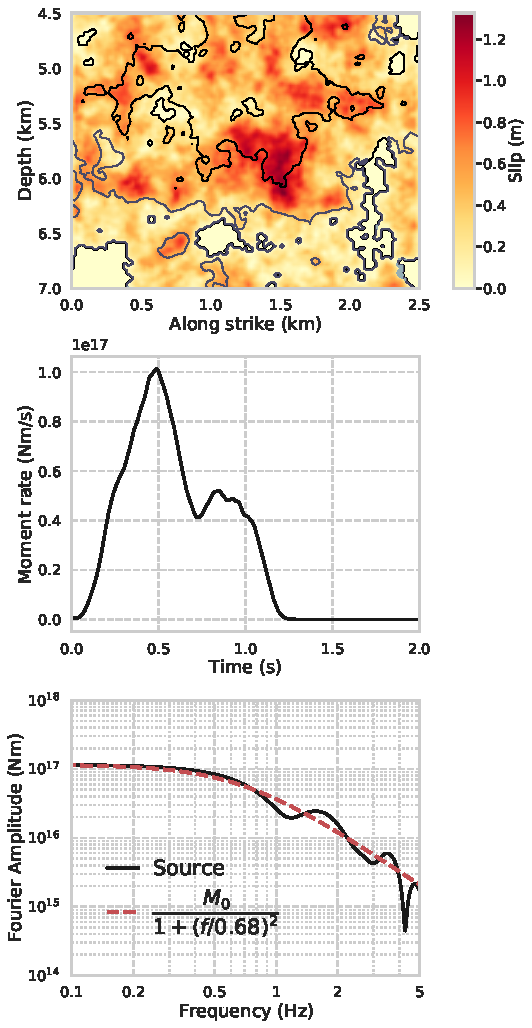
\includegraphics[width=0.9\textwidth,height=0.9\textheight,keepaspectratio]{figures/figure_highf_3.pdf}
  \caption{Source models used in this study. Sources 1, 2 and 3 (from left to right in the first row) are characterized by their hypocentral depths at 5, 5.5 and 6 km, respectively. The contours represent rupture time at a 0.4 s interval starting from 0. Source 1 is the default source model used elsewhere in this paper.}
  \label{fig:highf-3}
\end{figure}
\clearpage

\begin{figure}[!ht]
  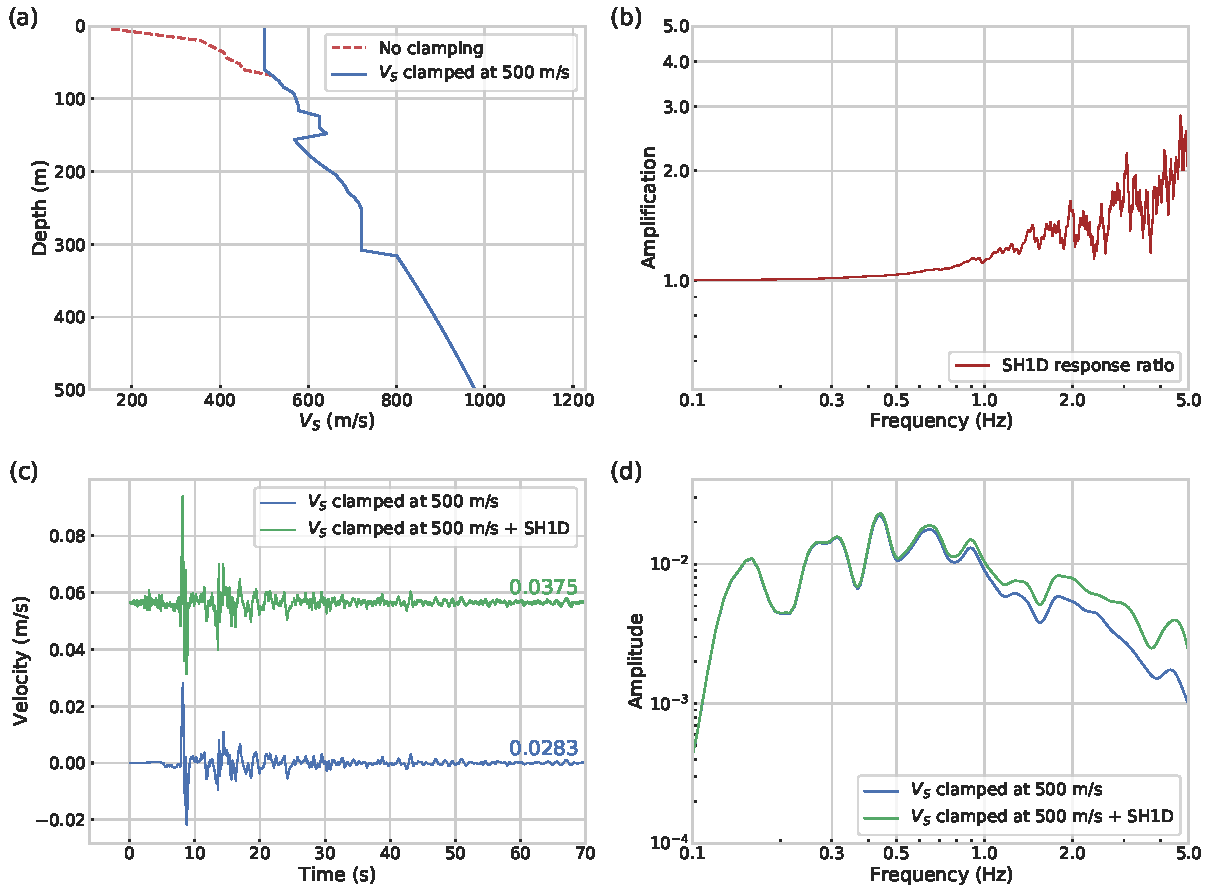
\includegraphics[width=0.9\textwidth,height=0.9\textheight,keepaspectratio]{figures/figure_highf_4.png}
  \caption{PGVs for sources 1, 2 and 3 (from left to right; see \cref{fig:highf-3}). The top and bottom rows represent the band-pass filtered results for 0.15-2.5 Hz and 2.5-5 Hz, respectively. The star denotes the epicenter.}
  \label{fig:highf-4}
\end{figure}
\clearpage

\begin{figure}[!ht]
  \centering
  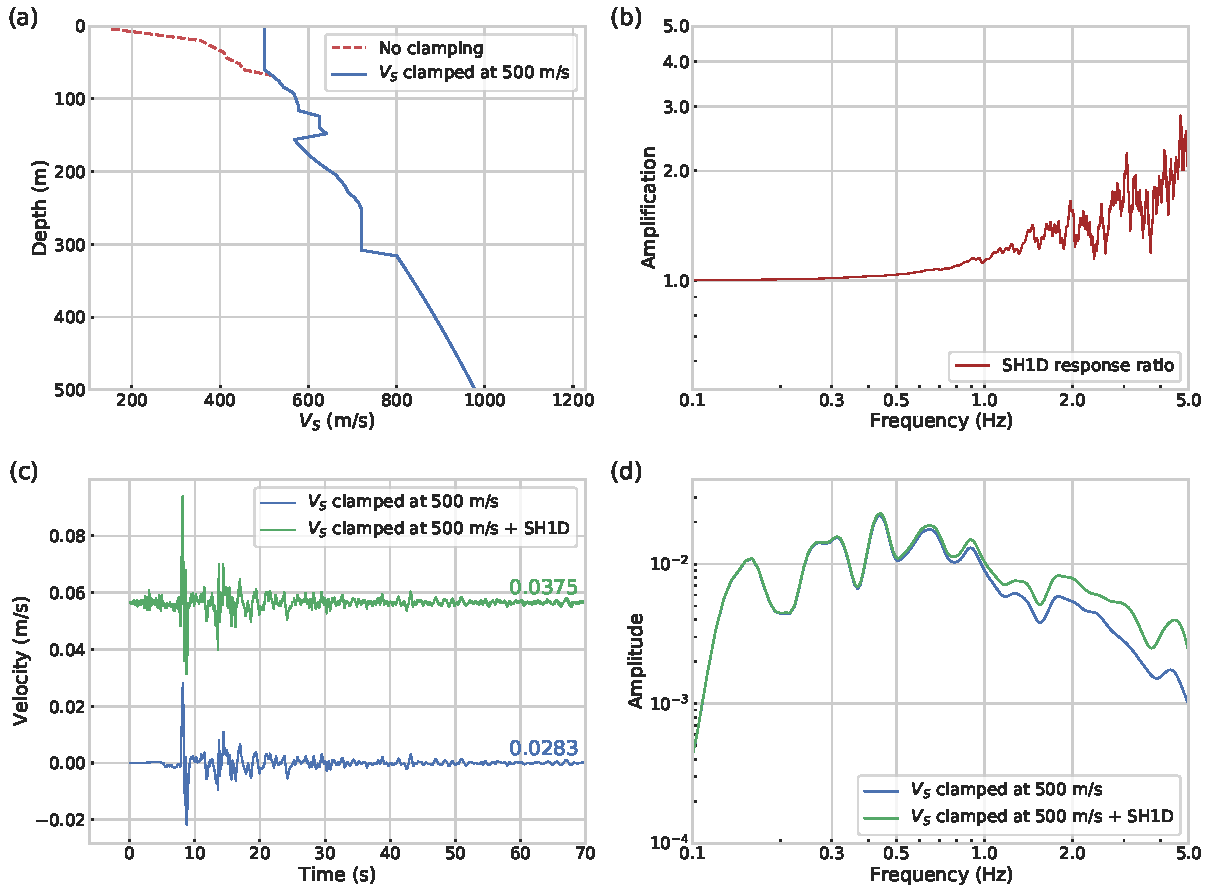
\includegraphics[width=0.9\textwidth,height=0.9\textheight,keepaspectratio]{figures/figure_highf_5.pdf}
  \caption{Illustration of the SH1D method used to include the effects of material with $V_S$ less than 500 m/s in our 3D simulations for an example site. (a) $V_S$ profile extracted from CVM-S (red dashed curve) and clamped at 500 m/s (blue). (b) SH1D response ratio between the profiles without clamping and with clamping of $V_S$ =500 m/s. (c) Synthetics from a 3D simulation using $V_S$=500m/s, with and without the SH1D response ratio. (d) Fourier amplitude spectra corresponding to the waveforms in (c).}
  \label{fig:highf-5}
\end{figure}
\clearpage


\begin{figure}[!ht]
  \centering
  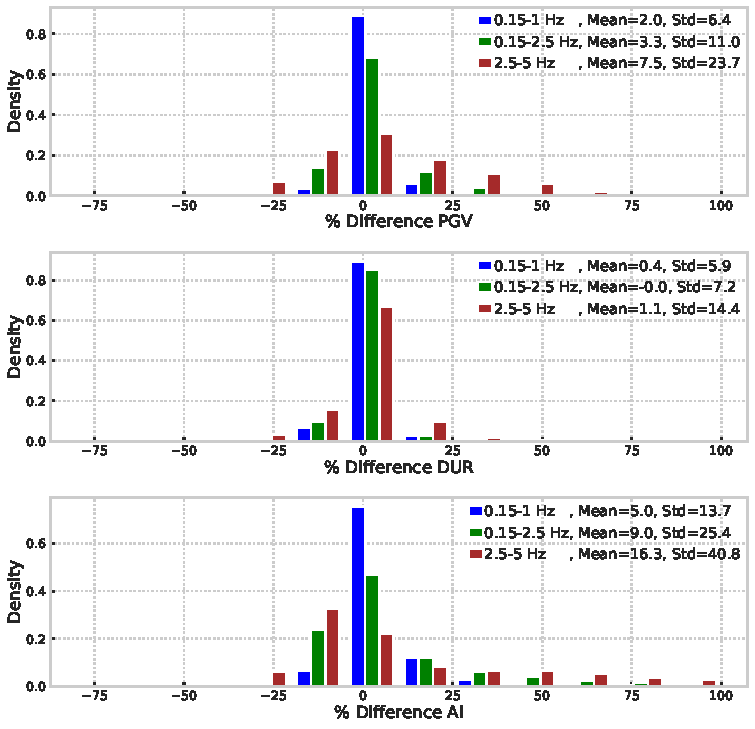
\includegraphics[width=0.9\textwidth,height=0.9\textheight,keepaspectratio]{figures/figure_highf_6.png}
  \caption{Comparison of interpolated PGVs measured at 259 stations, depicted by triangles, for (a) data and (b) synthetics using our reference model (including topography, 1000 m shallow velocity refinement and frequency-dependent attenuation $Q_S=0.1V_Sf^{0.6}$, $Q_P=2Q_S$). The star denotes the epicenter. (c) PGV against $R_{hypo}$ for data and synthetics. The left and right columns show band-limited results for 0.15-2.5 Hz, and 2.5-5 Hz, respectively.
  }
  \label{fig:highf-6}
\end{figure}
\clearpage

\begin{figure}[!ht]
  \centering
  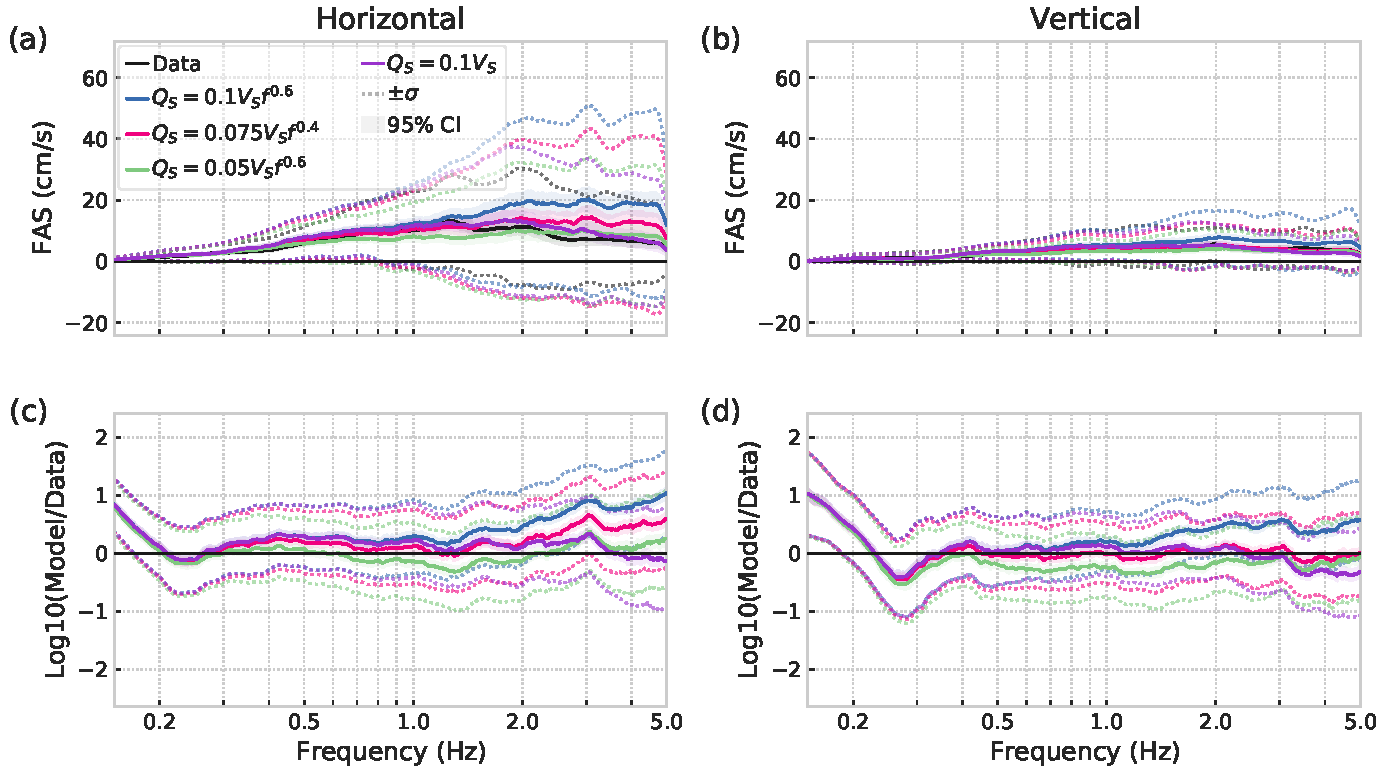
\includegraphics[width=0.9\textwidth,height=0.9\textheight,keepaspectratio]{figures/figure_highf_7.png}
  \caption{Percent difference of PGV (the first row) and DUR (the second row) at the surface determined by the model with topography and the model without topography for (left) 0.15-1 Hz, (center) 1-2.5 Hz, and (right) 2.5-5 Hz. The star denotes the epicenter.
  }
  \label{fig:highf-7}
\end{figure}
\clearpage

\begin{figure}[!ht]
  \centering
  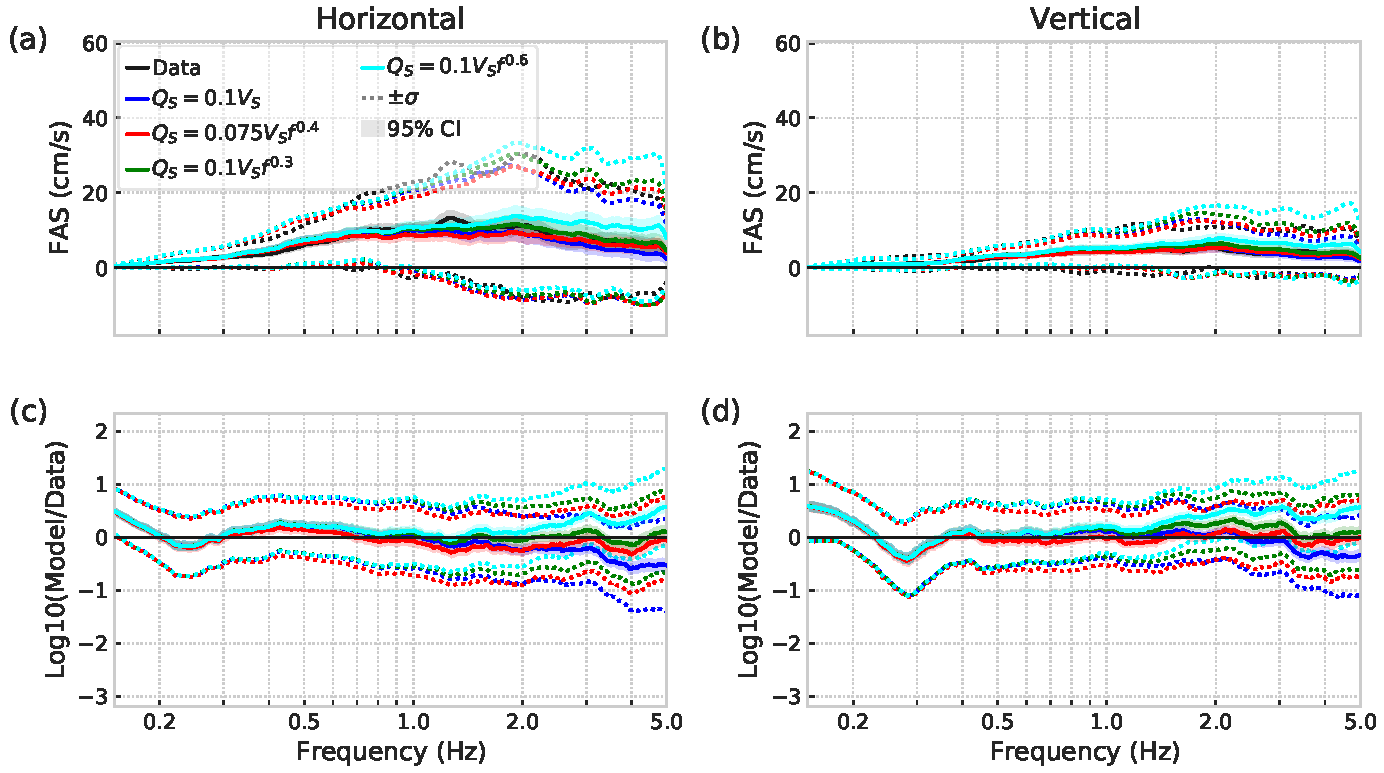
\includegraphics[width=0.9\textwidth,height=0.9\textheight,keepaspectratio]{figures/figure_highf_8.pdf}
  \caption{The FAS computed from records and models with various attenuation models. The left (right) row shows horizontal (vertical) component. The top row shows the FAS amplitudes and the bottom show FAS bias between models and records, calculated as 10-based log between simutation results and data. All models are based on the reference model except for different attenuation models. The solid line is the median FAS over all 259 stations; the shade depicts the 95\% confidence interval (CI) and the dashed lines denote one standard deviation centered at the median.
  }
  \label{fig:highf-8}
\end{figure}
\clearpage

\begin{figure}[!ht]
  \centering
  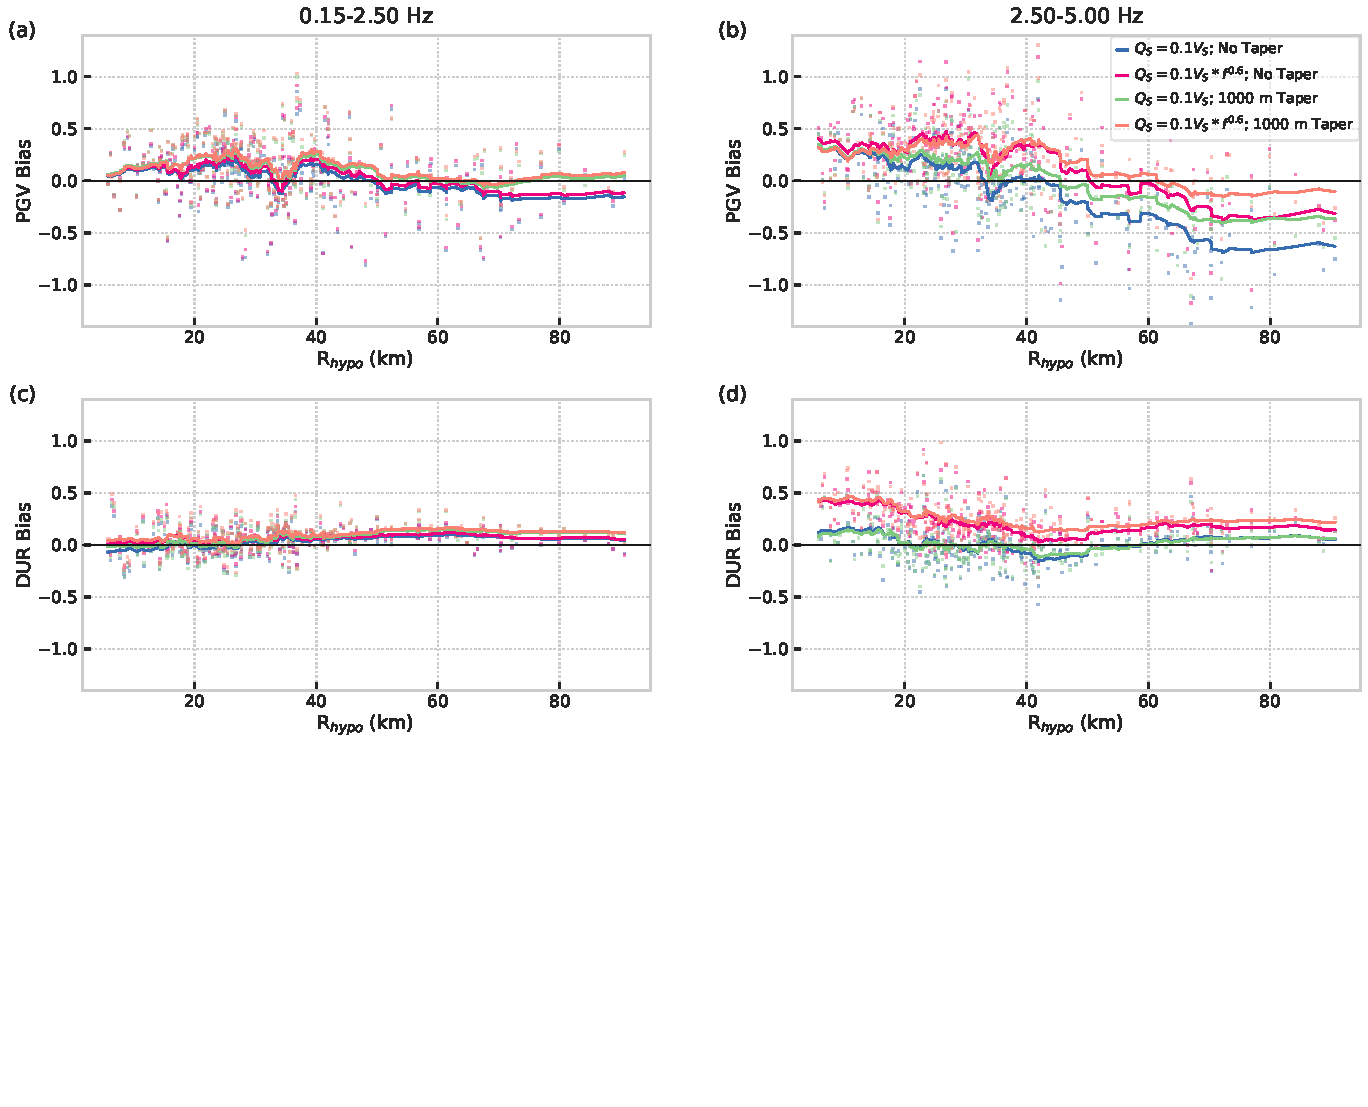
\includegraphics[width=0.9\textwidth,height=0.9\textheight,keepaspectratio]{figures/figure_highf_9.png}
  \caption{Spatial distribution of the bias in PGV band pass filtered between 2.5 and 5 Hz. The bias values are computed as the base 10 logarithm of the ratio between simulations and records at each validation site. Positive values represents overprediction in the simulation, and negative values indicate otherwise. (d) Moving average of the bias of PGV using a 20-point window from the three $Q$ models versus hypocentral distance.
  }
  \label{fig:highf-9}
\end{figure}
\clearpage

\begin{figure}[!ht]
  \centering
  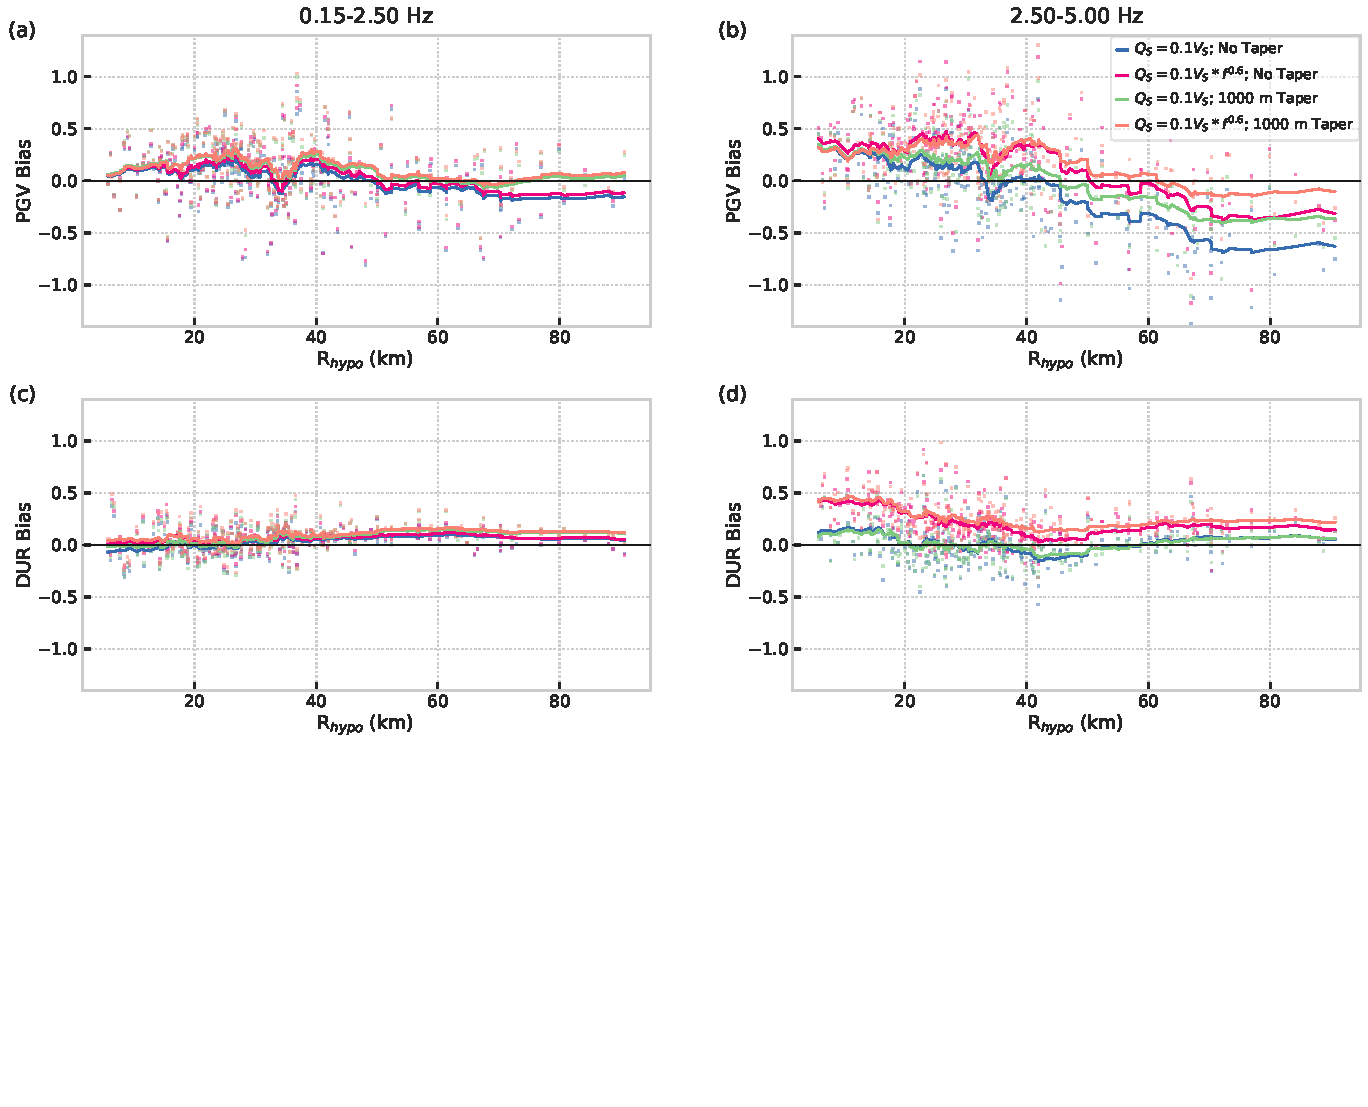
\includegraphics[width=0.9\textwidth,height=0.9\textheight,keepaspectratio]{figures/figure_highf_10.pdf}
  \caption{Bias of PGV and DUR in 0.15-2.5 Hz and 2.5-5 Hz at all 259 stations. The bias is calculated in the same way as \Cref{fig:highf-9}.
  }
  \label{fig:highf-10}
\end{figure}
\clearpage

\begin{figure}[!ht]
  \centering
  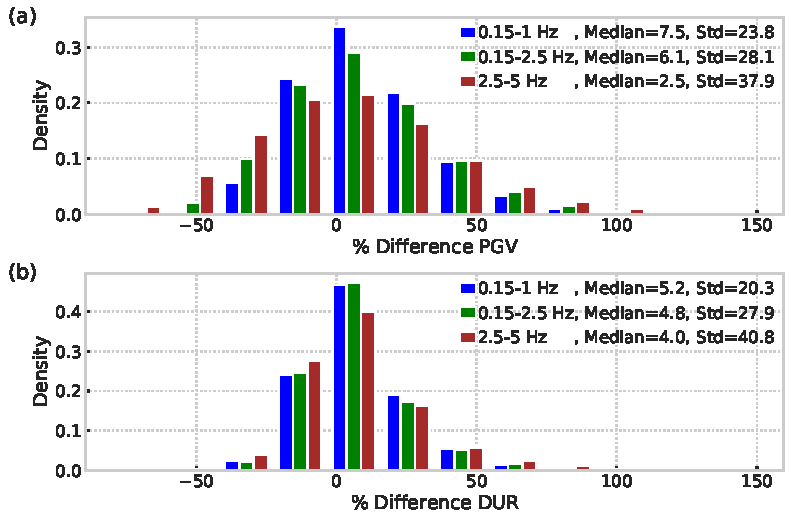
\includegraphics[width=0.9\textwidth,height=0.9\textheight,keepaspectratio]{figures/figure_highf_11.png}
  \caption{Comparison of PGV (top) and DUR (bottom) at the surface from the model including SSH with $\sigma = 5\%$ and $a = 5000$ m versus the reference model. The left and right columns are for bandwidths 0.15-2.5 Hz and 2.5-5 Hz, respectively. The colormap indicates the percent difference, calculated in the same way as \Cref{fig:highf-7}, between the model with SSH and the model without SSH. The star depicts the epicenter.
  }
  \label{fig:highf-11}
\end{figure}
\clearpage

\begin{figure}[!ht]
  \centering
  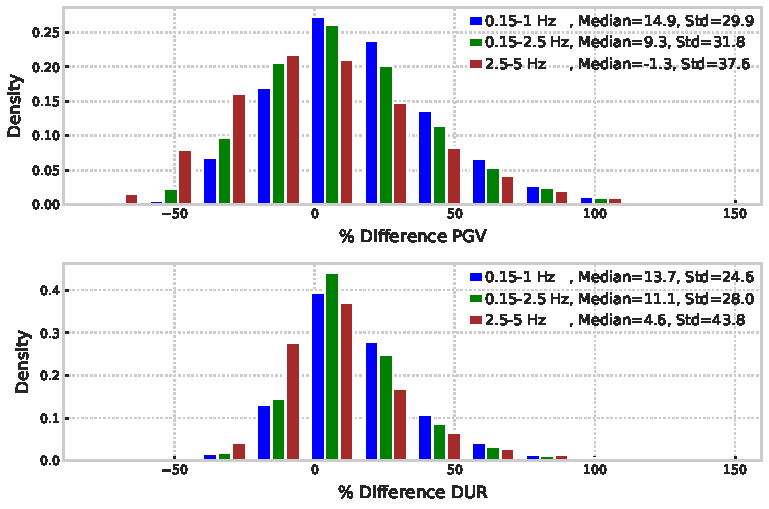
\includegraphics[width=0.9\textwidth,height=0.9\textheight,keepaspectratio]{figures/figure_highf_12.pdf}
  \caption{Probability density histogram of the difference between the model with SSH ($\sigma = 5\%$ and $a = 5000$ m) and the reference model without SSHs. The definition of percent difference (x-axis) is the same as in \Cref{fig:highf-7}.
  }
  \label{fig:highf-12}
\end{figure}
\clearpage

\begin{figure}[!ht]
  \centering
  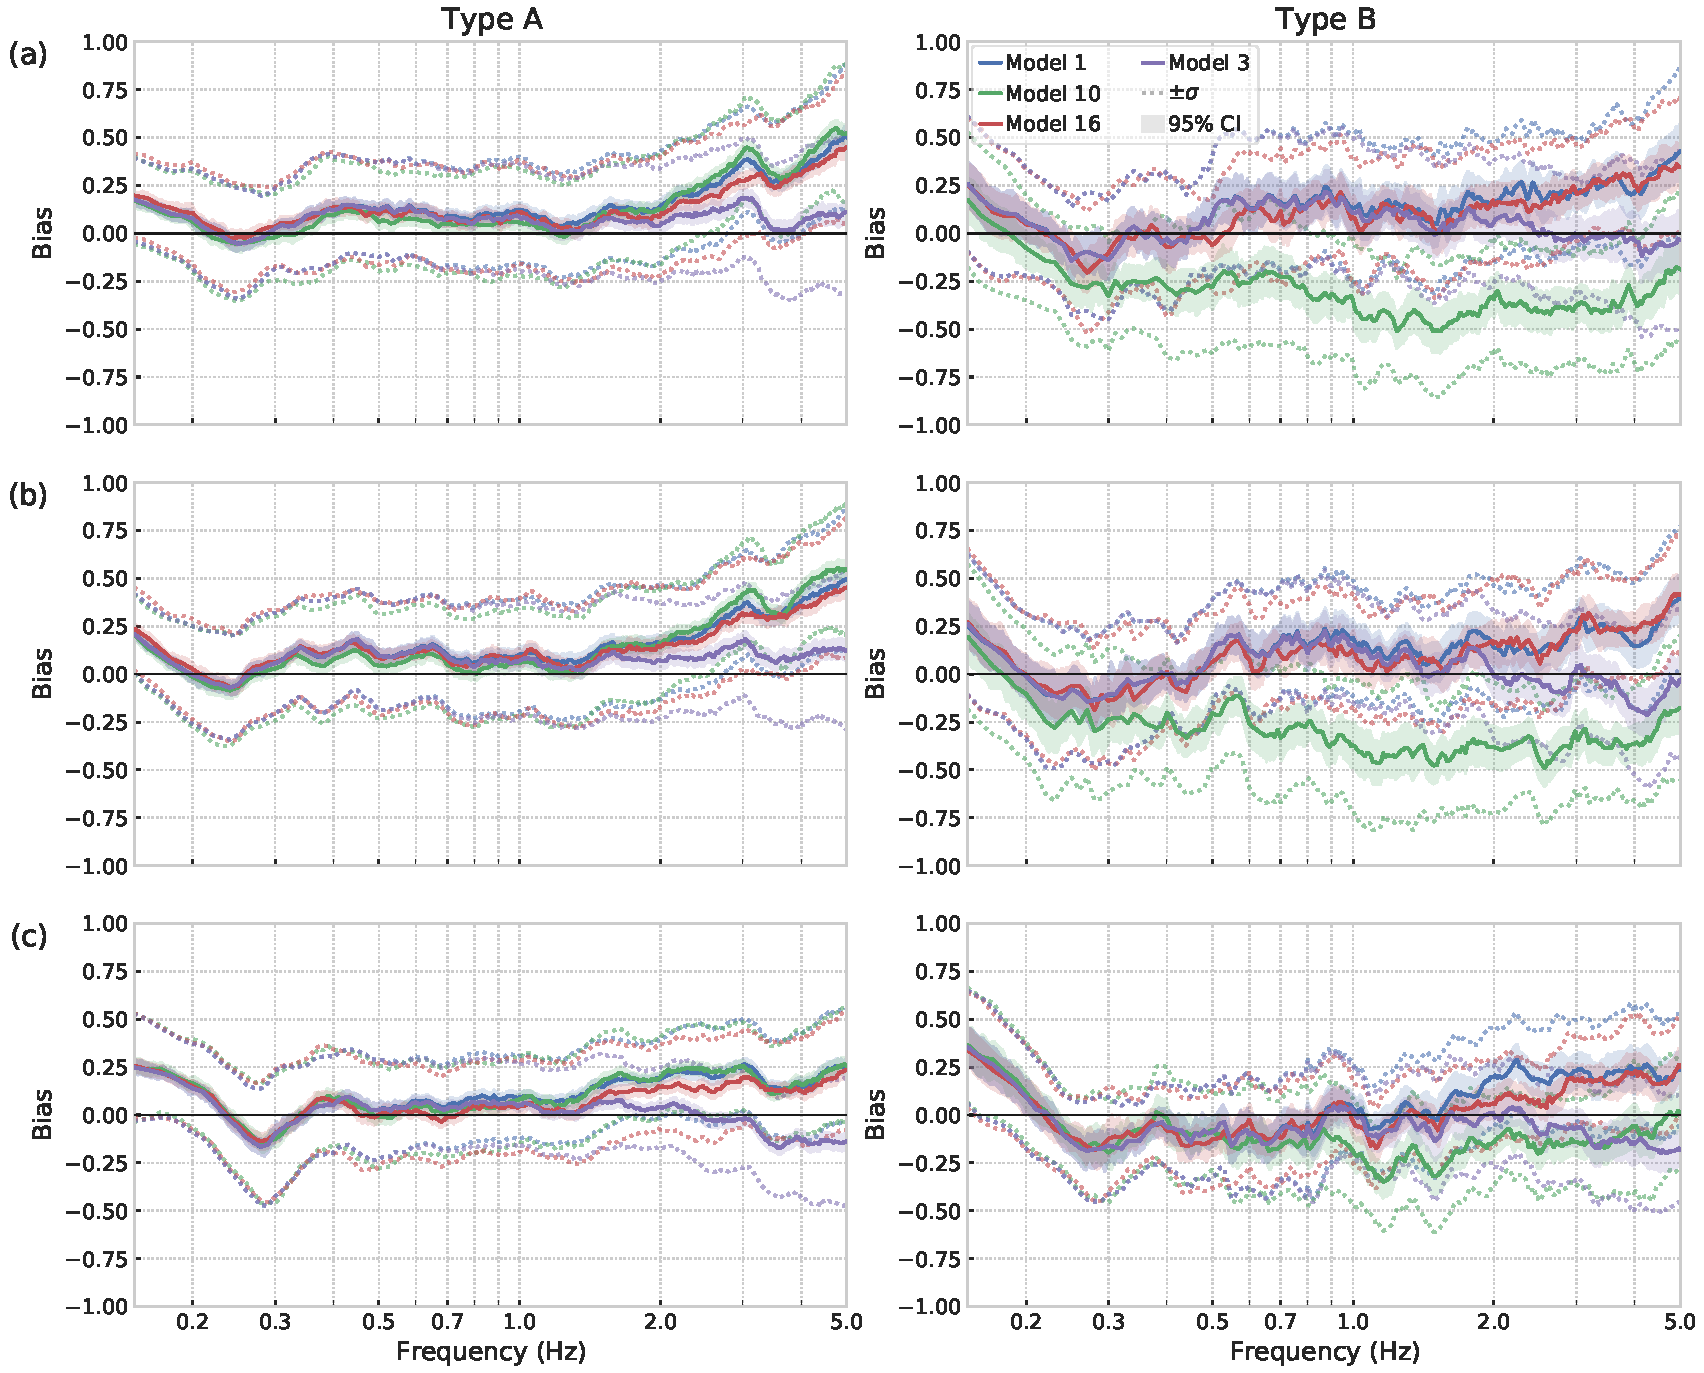
\includegraphics[width=0.9\textwidth,height=0.9\textheight,keepaspectratio]{figures/figure_highf_13.pdf}
  \caption{Bias of FAS on the (a) east-west, (b) north-south and (c) vertical components, calculated from models labeled by their IDs. A positive (negative) value depicts overprediction (underprediction). The left column shows type A sites, which are well constrained by geological information and right right column shows type (B) sites which are poorly constrained in CVM-S. The solid line is the median of FAS, where the narrow band is the 95\% confidence interval of the median, and the dashed lines depict the standard deviation centered at the median.
  }
  \label{fig:highf-13}
\end{figure}
\clearpage

\begin{figure}[!ht]
  \centering
  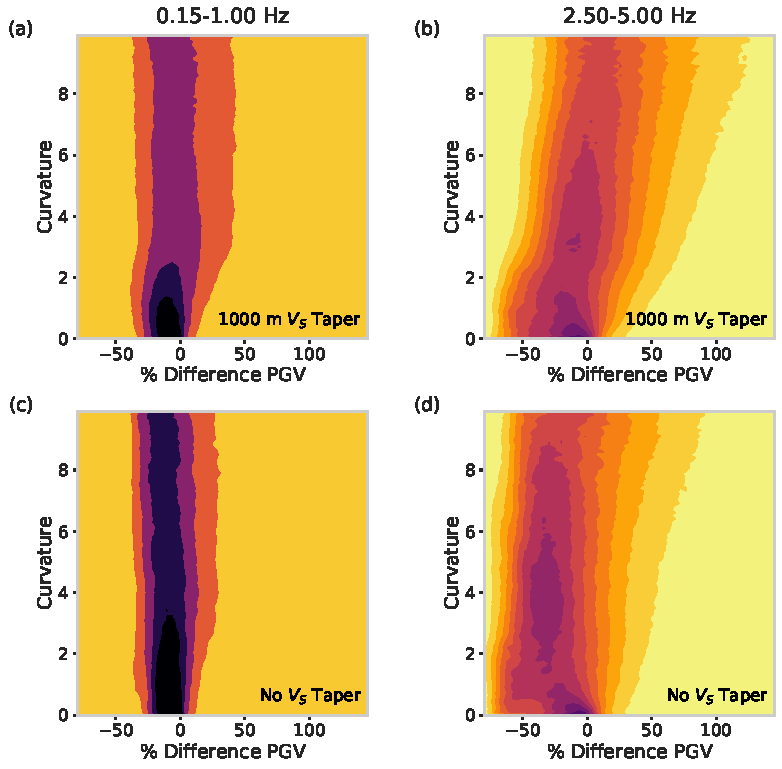
\includegraphics[width=0.9\textwidth,height=0.9\textheight,keepaspectratio]{figures/figure_highf_14.pdf}
  \caption{
 Density of PGV change for models with topography relative to models without topography for bandwidths of (left column) 0.15-2.5 Hz and (right column) 2.5-5 Hz, and models with (top row) and (bottom row) without modified shallow velocities. The y-axis depicts topographic curvature smoothed using a 2-D window of 640 m $\times$ 640 m. Values toward the top right (bottom left) denote strong amplification at steep areas (deamplification at flat areas). Note that density intervals do not correspond to constant bin sizes.}
  \label{fig:highf-14}
\end{figure}
\clearpage


\begin{figure}[!ht]
  \centering
  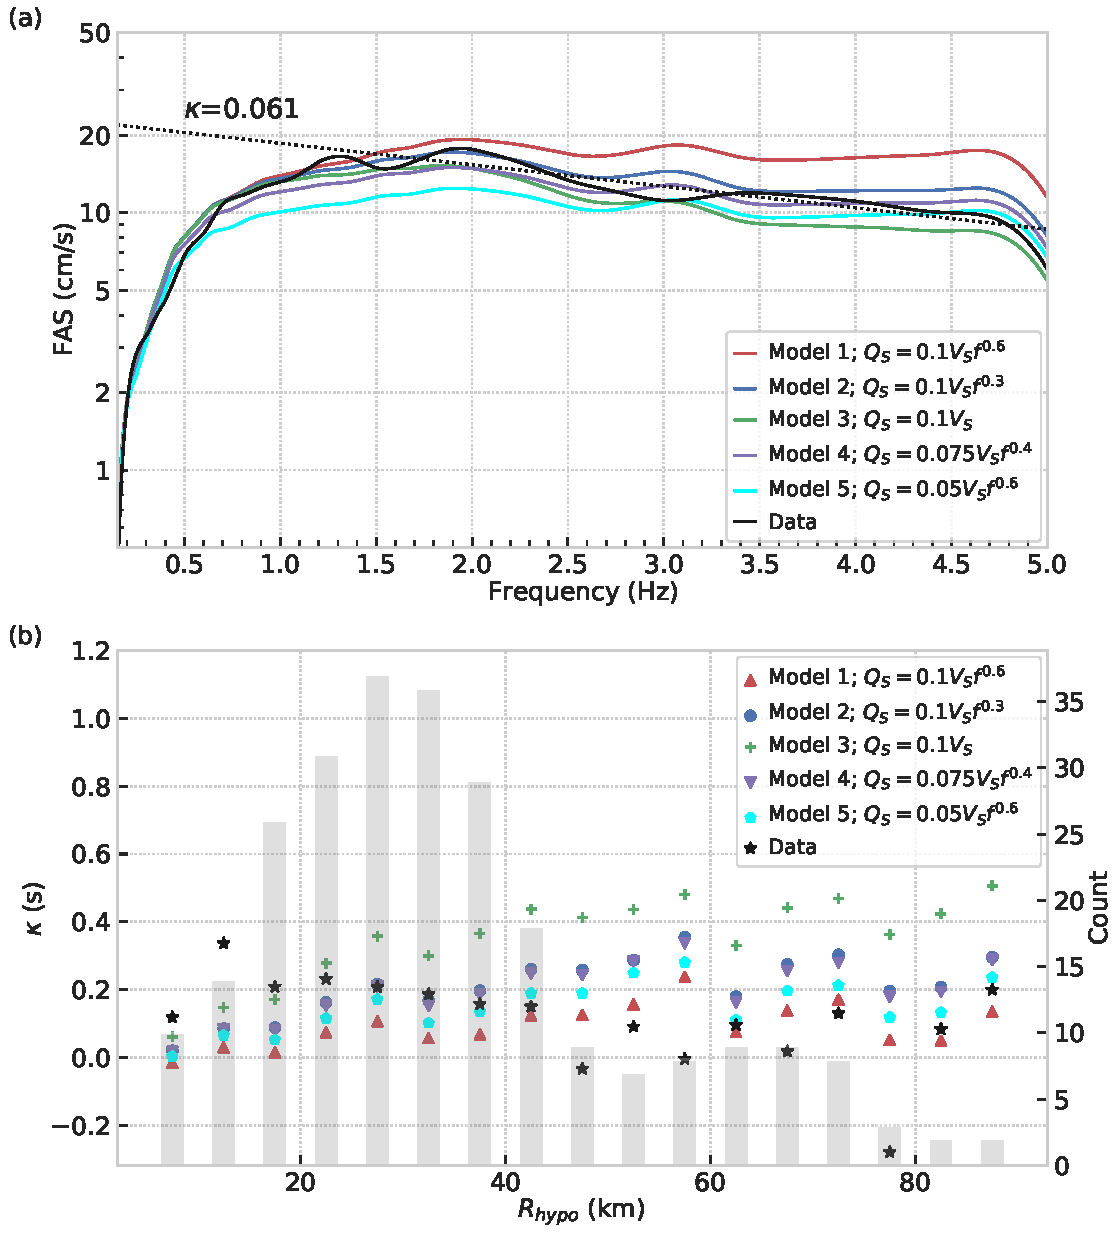
\includegraphics[width=0.9\textwidth,height=0.9\textheight,keepaspectratio]{figures/figure_highf_15.pdf}
  \caption{$\kappa$ values calculated for data and different $Q(f)$ models from the FAS between 2 and 5 Hz. (a) FAS staked over all stations for data and for 5 models (labels denote model ID, see \cref{tab:highf-2}, as well as the attenuation model for $Q_s$. All models use $Q_p$ = $2Q_s$. We find an average $\kappa$ value of 0.061 for the data. (b) Average $\kappa$ values calculated at stations binned in 5 km intervals (count) for data and models from (a).
  }
  \label{fig:highf-15}
\end{figure}
\clearpage



%% supplement
\setcounter{table}{0}
\setcounter{figure}{0}
\numberwithin{figure}{chapter}
\numberwithin{table}{chapter}
\renewcommand{\thetable}{S\arabic{chapter}.\arabic{table}}
\renewcommand{\thefigure}{S\arabic{chapter}.\arabic{figure}}
\newpage
\section*{Supplementary Materials}\label{highf:supplement}
\addcontentsline{toc}{section}{\protect\numberline{}Supplementary Materials}

\subsection{3D Simulation with Minimum $V_S$ of 200 m/s}\label{highf:vs200} 
\purple{We performed one 3D simulation using the CVM-S with minimum $V_S$ clamped at 200 m/s to verify the accuracy of the correction technique using the SH1D method by applying on another 3D simulation with minimum $V_S$ clamped at 500 m/s.}

\purple{The original version of AWP employs a spatially uniform grid over the entire domain, where the minimum velocity determines the grid spacing, resulting in significant over-discretization in high-velocity areas. \citet{nieFourthOrderStaggered2017} developed a method that supports discontinuous mesh (DM) for the 3D staggered-grid finite-difference scheme in AWP. The wavefields are exchanged within an overlap zone between two media partitions with a factor-of-three change in grid spacing, which significantly reduces the number of grid points needed in high-velocity regions and thereby improves the efficiency. The tremendously improved efficiency from DM allows us to lower the minimum $V_S$ to 200 m/s using a flat free surface. The simulated domain (\Cref{tab:highf-1}) is discretized into three partitions: 1) dx=8 m from the surface to 1,472 m, 2) dx=24 m between 1,472 m and 10,336 m, and 3) dx=72 m at deeper levels.} 

\purple{\Cref{fig:highf-S1} shows the FAS bias of the two 3D simulations with minimum $V_S$ of 200 m/s and 500 m/s respectively. The SH1D response ratio is calculated using the same profiles, with minimum $V_S$ clamped correspondingly, at all stations and applied upon the 500 m/s simulation. It is noticable that reducing minimum $V_S$ yields minimal difference in the vertical components. For horizontal components, the SH1D correction matches the minimum $V_S$ of 200 m/s simulation decently below about 2.5 Hz, and tends to overpredict moderately above that. Considering the potential inaccuracy toward the high end of the frequency band due to the aggressive usage of 5 points per minimum S-wavelength , we deem the SH1D correction reasonably accounts for the low-velocity effects.}

%we compared the response of Model 2 (minimum $V_S$ of 200 m/s) to a variation of Model 2 with minimum $V_S$ of 500 m/s (\cref{fig:highf-5}). As expected, the largest effects are observed above the basin areas with the lowest near-surface velocities. At frequencies below 1 Hz, the PGV amplification is generally concentrated in basins with low near-surface $V_S$. However, as frequency increases, the amplification in PGV extends to the surrounding low-altitude areas, including mountain valleys. For 2.5-5 Hz seismic waves, deamplification starts to show up in the mountain regions, likely due to entrapment and attenuation of seismic energy in the basin areas. DUR is relatively less affected by reducing the minimum $V_S$, compared to PGV and AI. As the effects of the near-surface velocities are somewhat similar for PGV and AI in pattern and amplitude. %Considering the similar patterns for the ground motions calculated for 0.15-1 Hz and 0.15-2.5 Hz, we will not show 0.15-2.5 Hz and AI in the subsequent plots of ground motion metrics.

\begin{figure}[!ht]
  \centering
  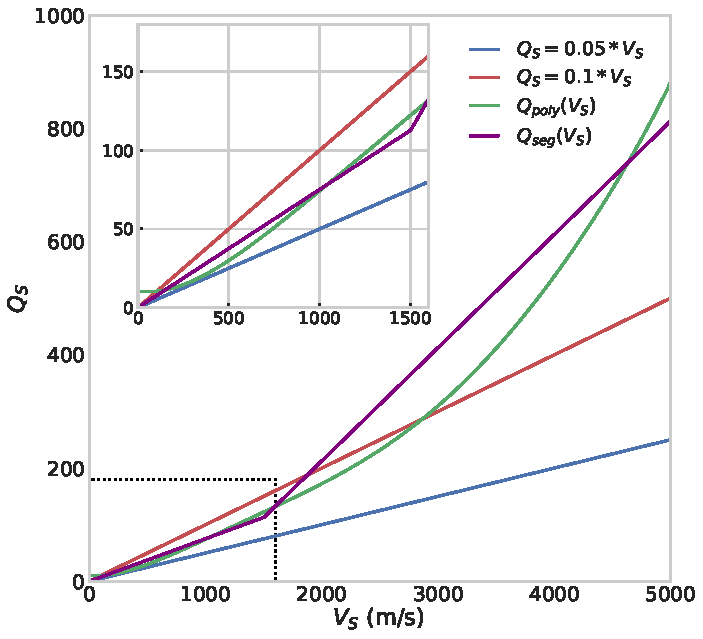
\includegraphics[width=0.9\textwidth,height=0.85\textheight,keepaspectratio]{figures/figure_highf_S1.pdf}
  \caption{
  \purple{The FAS bias, calculated as 10-based log ratio, between simulated synthetics with minimum $V_S$ clamped at 200 m/s (blue) or 500 m/s (green) and records. The FAS bias from the latter 500 m/s minimum $V_S$ simulation convolved with SH1D response ratio is shown in purple. (a) and (b) show two horizontal components and (c) show the vertical component. A positive bias means overprediction and a negative value means the opposite. The solid line is the median FAS bias over all 259 stations; the shade depicts the 95\% confidence interval (CI) and the dashed lines denote one standard deviation centered at the median.}
  }
  \label{fig:highf-S1}
\end{figure}
\clearpage

\begin{figure}[!ht]
  \centering
  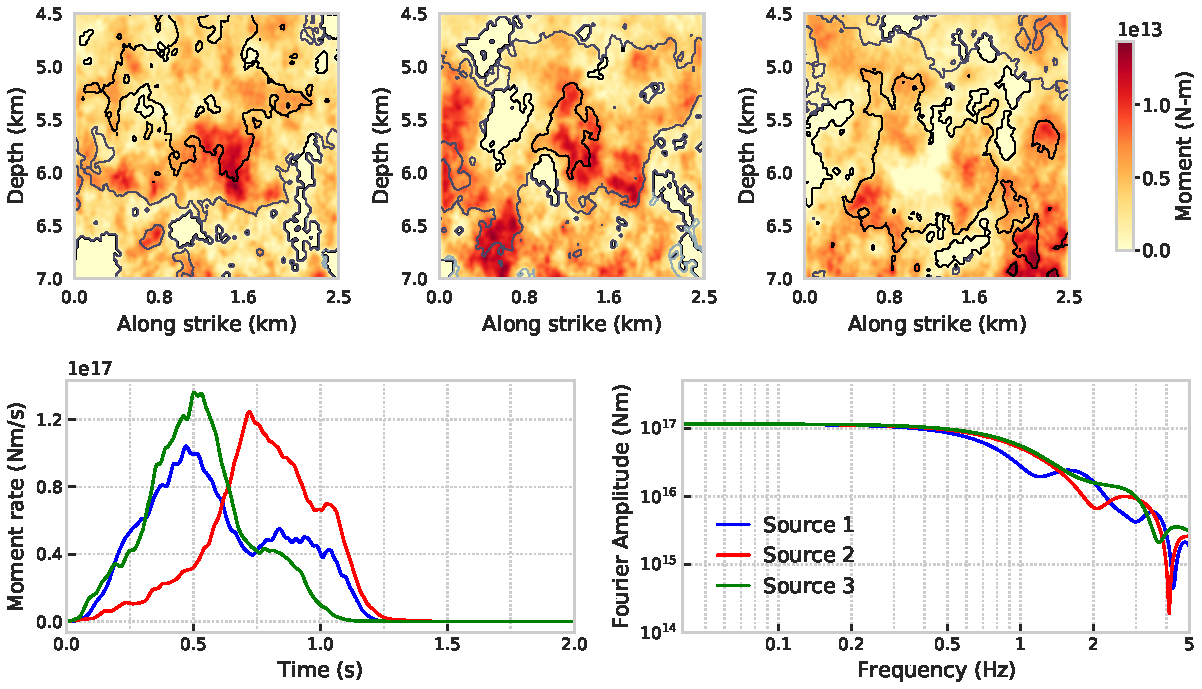
\includegraphics[width=0.9\textwidth,height=0.9\textheight,keepaspectratio]{figures/figure_highf_S2.pdf}
  \caption{Probability density histogram of the PGV difference between the model with various SSH models and the reference model without SSHs. The definition of percent difference (x-axis) is the same as in \Cref{fig:highf-11}.
  }
  \label{fig:highf-S2}
\end{figure}
\clearpage

\begin{figure}[!ht]
  \centering
  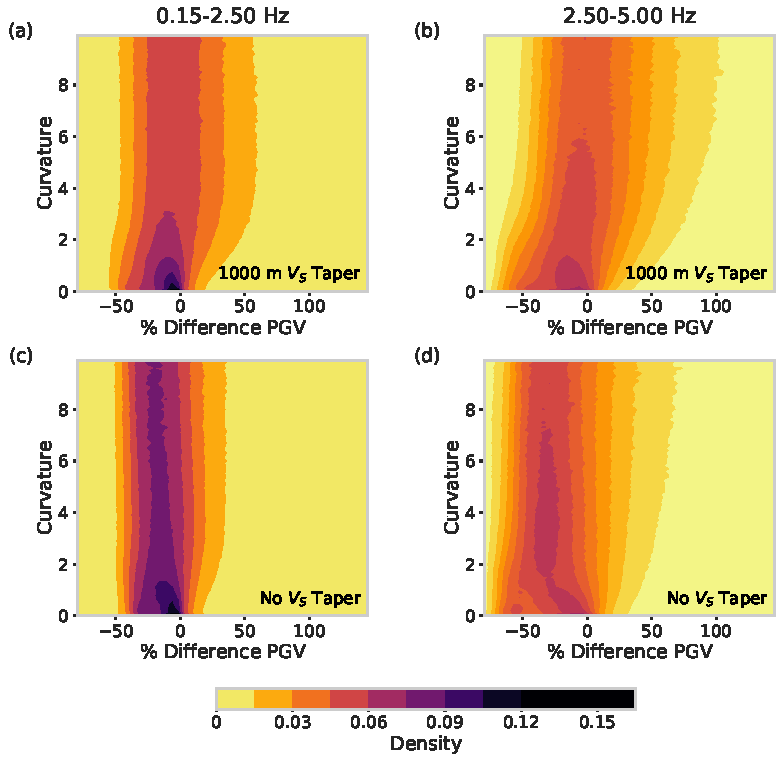
\includegraphics[width=0.9\textwidth,height=0.9\textheight,keepaspectratio]{figures/figure_highf_S3.pdf}
  \caption{
  Density of PGV change for models with topography relative to models without topography for bandwidths of (left column) 0.15-2.5 Hz and (right column) 2.5-5 Hz, and models with (top row) and (bottom row) without modified shallow velocities. The y-axis depicts topographic curvature smoothed using a 2-D window of 120 m $\times$ 120 m. Values toward the top right (bottom left) denote strong amplification at steep areas (deamplification at flat areas). Note that density intervals do not correspond to constant bin sizes.
  }
  \label{fig:highf-S3}
\end{figure}
\clearpage




\renewcommand{\thetable}{\arabic{table}}
\renewcommand{\thefigure}{\arabic{figure}}

\numberwithin{figure}{chapter}
\numberwithin{table}{chapter}

%\endrefsection